
\documentclass[a4paper,11pt]{article}%,twocolumn
%% packages

\usepackage{blindtext} % needed for creating dummy text passages
%\usepackage{ngerman} % needed for German default language
\usepackage{amsmath} % needed for command eqref
\usepackage{amssymb} % needed for math fonts
\usepackage[colorlinks=true,breaklinks]{hyperref} % needed for creating hyperlinks in the document, the option colorlinks=true gets rid of the awful boxes, breaklinks breaks lonkg links (list of figures), and ngerman sets everything for german as default hyperlinks language
\usepackage[hyphenbreaks]{breakurl} % ben�tigt f�r das Brechen von URLs in Literaturreferenzen, hyphenbreaks auch bei links, die �ber eine Seite gehen (mit hyphenation).
\usepackage{xcolor}
\definecolor{c1}{rgb}{0,0,1} % blue
\definecolor{c2}{rgb}{0,0.3,0.9} % light blue
\definecolor{c3}{rgb}{0.3,0,0.9} % red blue
\hypersetup{
    linkcolor={c1}, % internal links
    citecolor={c2}, % citations
    urlcolor={c3} % external links/urls
}
%\usepackage{cite} % needed for cite
\usepackage[square,authoryear]{natbib} % needed for cite and abbrvnat bibliography style
\usepackage[nottoc]{tocbibind} % needed for displaying bibliography and other in the table of contents
\usepackage{graphicx} % needed for \includegraphics 
\usepackage{longtable} % needed for long tables over pages
\usepackage{bigstrut} % needed for the command \bigstrut
\usepackage{enumerate} % needed for some options in enumerate
%\usepackage{todonotes} % needed for todos
\usepackage{makeidx} % needed for creating an index
\makeindex
\usepackage{gensymb}
\usepackage{url}
\usepackage{psfrag}
\usepackage{multirow}
\usepackage{subfigure}
%% page settings

\usepackage[top=20mm, bottom=20mm,left=15mm,right=15mm]{geometry} % needed for page border settings
\parindent=0mm % for space of first line of new text block
\sloppy % for writing with hyphenless justification (tries to)
\hyphenation{} % use hyphenation of tolerance parametershttp://www.jr-x.de/publikationen/latex/tipps/zeilenumbruch.html
\hyphenpenalty=10000
\exhyphenpenalty=10000
\usepackage{fancyhdr} % needed for head and foot options
%% my macros

%% Text fomats
\newcommand{\tbi}[1]{\textbf{\textit{#1}}}

%% Math fonts
\newcommand{\bbA}{\mathbb{A}}
\newcommand{\bbB}{\mathbb{B}}
\newcommand{\bbC}{\mathbb{C}}
\newcommand{\bbD}{\mathbb{D}}
\newcommand{\bbE}{\mathbb{E}}
\newcommand{\bbF}{\mathbb{F}}
\newcommand{\bbG}{\mathbb{G}}
\newcommand{\bbH}{\mathbb{H}}
\newcommand{\bbI}{\mathbb{I}}
\newcommand{\bbJ}{\mathbb{J}}
\newcommand{\bbK}{\mathbb{K}}
\newcommand{\bbL}{\mathbb{L}}
\newcommand{\bbM}{\mathbb{M}}
\newcommand{\bbN}{\mathbb{N}}
\newcommand{\bbO}{\mathbb{O}}
\newcommand{\bbP}{\mathbb{P}}
\newcommand{\bbQ}{\mathbb{Q}}
\newcommand{\bbR}{\mathbb{R}}
\newcommand{\bbS}{\mathbb{S}}
\newcommand{\bbT}{\mathbb{T}}
\newcommand{\bbU}{\mathbb{U}}
\newcommand{\bbV}{\mathbb{V}}
\newcommand{\bbW}{\mathbb{W}}
\newcommand{\bbX}{\mathbb{X}}
\newcommand{\bbY}{\mathbb{Y}}
\newcommand{\bbZ}{\mathbb{Z}}
\usepackage[ framed, numbered]{matlab-prettifier}%framed,%
\usepackage{listings}
\usepackage{physics}
\usepackage{pdfpages}
\usepackage[toc,page]{appendix}
\usepackage{float}
\usepackage{hyperref}

% for code
\usepackage{listings}
\usepackage{color}
% Define colors
\definecolor{codegreen}{rgb}{0,0.6,0}
\definecolor{codegray}{rgb}{0.5,0.5,0.5}
\definecolor{codepurple}{rgb}{0.58,0,0.82}
\definecolor{backcolour}{rgb}{0.95,0.95,0.92}
% Setup the listings package
\lstset{
    backgroundcolor=\color{backcolour},   
    commentstyle=\color{codegreen},
    keywordstyle=\color{magenta},
    numberstyle=\tiny\color{codegray},
    stringstyle=\color{codepurple},
    basicstyle=\footnotesize,
    breakatwhitespace=false,         
    breaklines=true,                 
    captionpos=b,                    
    keepspaces=true,                 
    numbers=left,                    
    numbersep=5pt,                  
    showspaces=false,                
    showstringspaces=false,
    showtabs=false,                  
    tabsize=2
}

\newenvironment{qanda}{\setlength{\parindent}{0pt}}{\bigskip}
\newcommand{\Q}{\bigskip\bfseries Q: }
\newcommand{\A}{\par\textbf{Answer: } \normalfont}

\begin{document}
\begin{titlepage}
\center % Center everything on the page

%-------------------------------------------------------------------------------------
%	HEADING SECTIONS
%------------------------------------------------------------------------------------
\textbf{\large Department of Electrical and Computer Engineering}\\[0.5cm]
\textbf{\Large University of Colorado at Boulder}\\[1cm]
\textbf{\large ECEN5623 - Real Time Embedded Systems }\\[2cm]

\includegraphics[width=0.3\textwidth]{figures/cu}\\[2cm]

	
%-------------------------------------------------------------------------------------
%	TITLE SECTION
%------------------------------------------------------------------------------------
\textbf{\Huge Exercise 5 }\\[0.2cm]



%----------------------------------------------------------------------------------------
%	MEMBERS SECTION
%----------------------------------------------------------------------------------------


\vfill

\textbf{\large Submitted by}\\[0.5cm]

{\large Parth | Jithedra}\\[0.5cm]	

%----------------------------------------------------------------------------------------
%	DATE SECTION
%----------------------------------------------------------------------------------------

\textbf{\large Submitted on}
\textbf{\Large \today} % Date, change the \today to a set date if you want to be precise

%----------------------------------------------------------------------------------------

\vfill % Fill the rest of the page with whitespace

\end{titlepage}


\pagebreak

\tableofcontents
\listoffigures
\listoftables
\vfill
\begin{center}
	\textbf{\textit{*PDF is clickable}}
\end{center}



\pagebreak
\begin{qanda}
	\section{Question 1}
	\begin{enumerate}
		\item[] \Q [10 points] Obtain a Logitech C200 or C270 camera or equivalent and
			verify that is detected by the DE1-SoC, Raspberry Pi or Jetson Board USB driver. You can check
			the camera out from eStore or purchase one of your own, or use another camera that has a compliant
			UVC driver. Use lsusb, lsmod and dmesg kernel driver configuration tool to make sure your
			Logitech C2xx USB camera is plugged in and recognized by your DE1-SoC, Raspberry Pi or Jetson
			(note that on the Jetson, it does not use driver modules, but rather a monolithic kernel image, so
			lsmod will not look the same as other Linux systems – see what you can find by exploring /cat/proc
			on you Jetson to find the camera USB device). For the Jetson, do lsusb | grep C200 (or C270) and
			prove to the TA (and more importantly yourself) with that output (screenshot) that your camera is
			recognized. For systems other than a Jetson, do lsmod | grep video and verify that the UVC driver is
			loaded as well (http://www.ideasonboard.org/uvc/ ). To further verify, or debug if you don’t see the
			UVC driver loaded in response to plugging in the USB camera, do dmesg | grep video or just dmesg
			and scroll through the log messages to see if your USB device was found. Capture all output and
			annotate what you see with descriptions to the best of your understanding.
			\A
			\textbf{Verify Camera Detection}
			\begin{enumerate}
				\item Check USB Devices:\\

				      Command: lsusb\\
				      This command lists all USB devices currently connected to the system. Running this in the terminal helps you identify whether the Logitech camera is physically recognized by the system. The output includes details like the device ID and the manufacturer, which can be used to confirm the presence of the camera.\\

				      \begin{figure}[H]
					      \centering
					      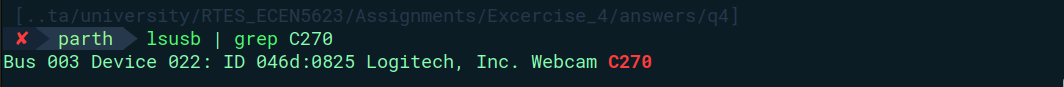
\includegraphics[scale=0.45]{figures/lsusb.png}
					      \caption{lsusb}
				      \end{figure}
				\item Verify UVC Driver Load:\\

				      Command: lsmod | grep video\\
				      Purpose: The lsmod command displays a list of loaded kernel modules, and piping this output to grep video filters the list to show only modules related to video, such as the UVC (USB Video Class) driver, often indicated by uvcvideo. This command verifies that the necessary driver for operating the camera is loaded in the system. The UVC driver is crucial because it provides generic support for USB video devices, ensuring that compliant cameras can work with a broad set of operating systems and applications without requiring proprietary drivers.

				      \begin{figure}[H]
					      \centering
					      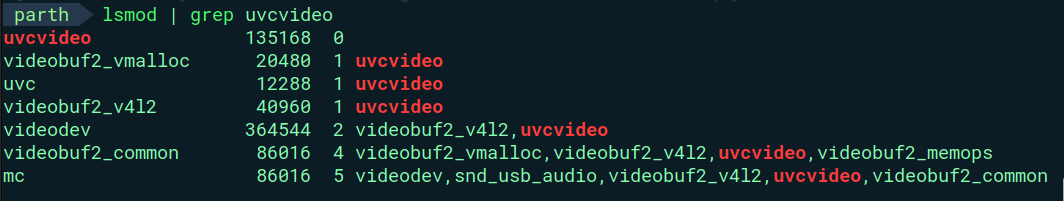
\includegraphics[scale=0.45]{figures/lsmod.png}
					      \caption{lsmod}
				      \end{figure}
				\item Inspect Kernel Messages:\\
				      Commands: dmesg | grep video and dmesg\\
				      Purpose: These commands are used to inspect kernel messages.
				      dmesg displays a log of system messages, including hardware detection, drivers loaded, and errors encountered during the boot process or while the system is running.
				      dmesg | grep video narrows down this log to entries related to video devices and drivers. This can reveal whether the camera was successfully initialized, recognized, and configured by the kernel, or if there were any issues during its detection process.
				      \begin{figure}[H]
					      \centering
					      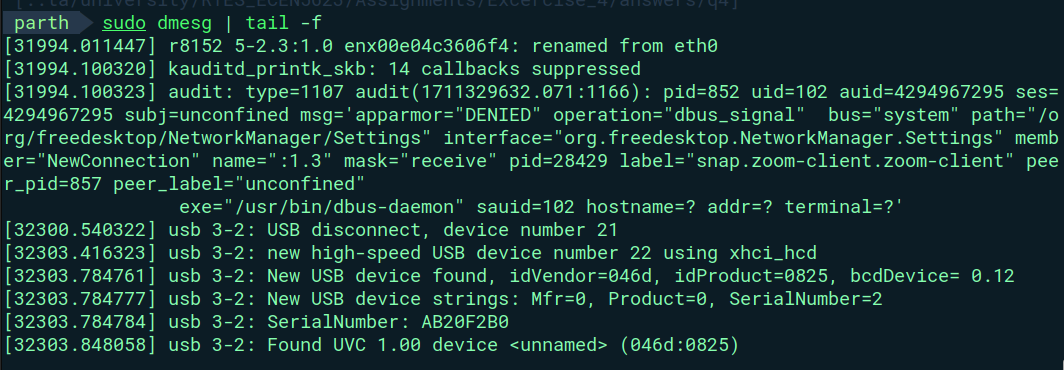
\includegraphics[scale=0.45]{figures/dmesg.png}
					      \caption{Kernel Message}
				      \end{figure}
			\end{enumerate}

	\end{enumerate}




	\section{Question 2}
	\begin{enumerate}
		\item[] \Q Option 2: Cheese
			If you do not have cheese, do sudo apt-get install cheese on your Jetson, Raspberry Pi or DE1-SoC
			board or other native Linux system. This should not only install nice camera capture GUI tools, but
			also the V4L2 API described well in this series of Linux articles - http://lwn.net/Articles/203924/ .
			Running cheese should provide an interactive camera control session for your Logitech C2xx camera
			– if you have issues connecting to your camera do a “man cheese” and specify your camera device
			file entry point (e.g. /dev/video0). Show that you tested your camera with a cheese screen dump and
			test photo.
			\A
			Install Cheese: Execute the following command:\\
			\begin{lstlisting}[language=sh]
sudo apt-get install cheese
			\end{lstlisting}
			\begin{figure}[H]
				\centering
				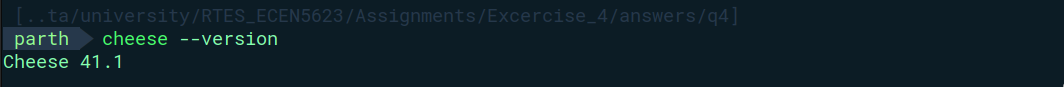
\includegraphics[scale=0.45]{figures/cheese_version.png}
				\caption{Cheese Version}
			\end{figure}

			Manual Device Selection: If Cheese does not automatically detect your camera, or if you encounter issues, you can specify the camera device file manually:

			Determine your camera's device file (/dev/video0 for the first detected video device). You can list video devices with ls /dev/video*.
			Launch Cheese with a specified device file by running: cheese --device=/dev/video0 (replace /dev/video0 with camera's device file if different).

			Screen Dump: screenshot of the Cheese application window showing the live camera feed with keyboard shortcut (e.g., PrtScn key).
			\begin{figure}[H]
				\centering
				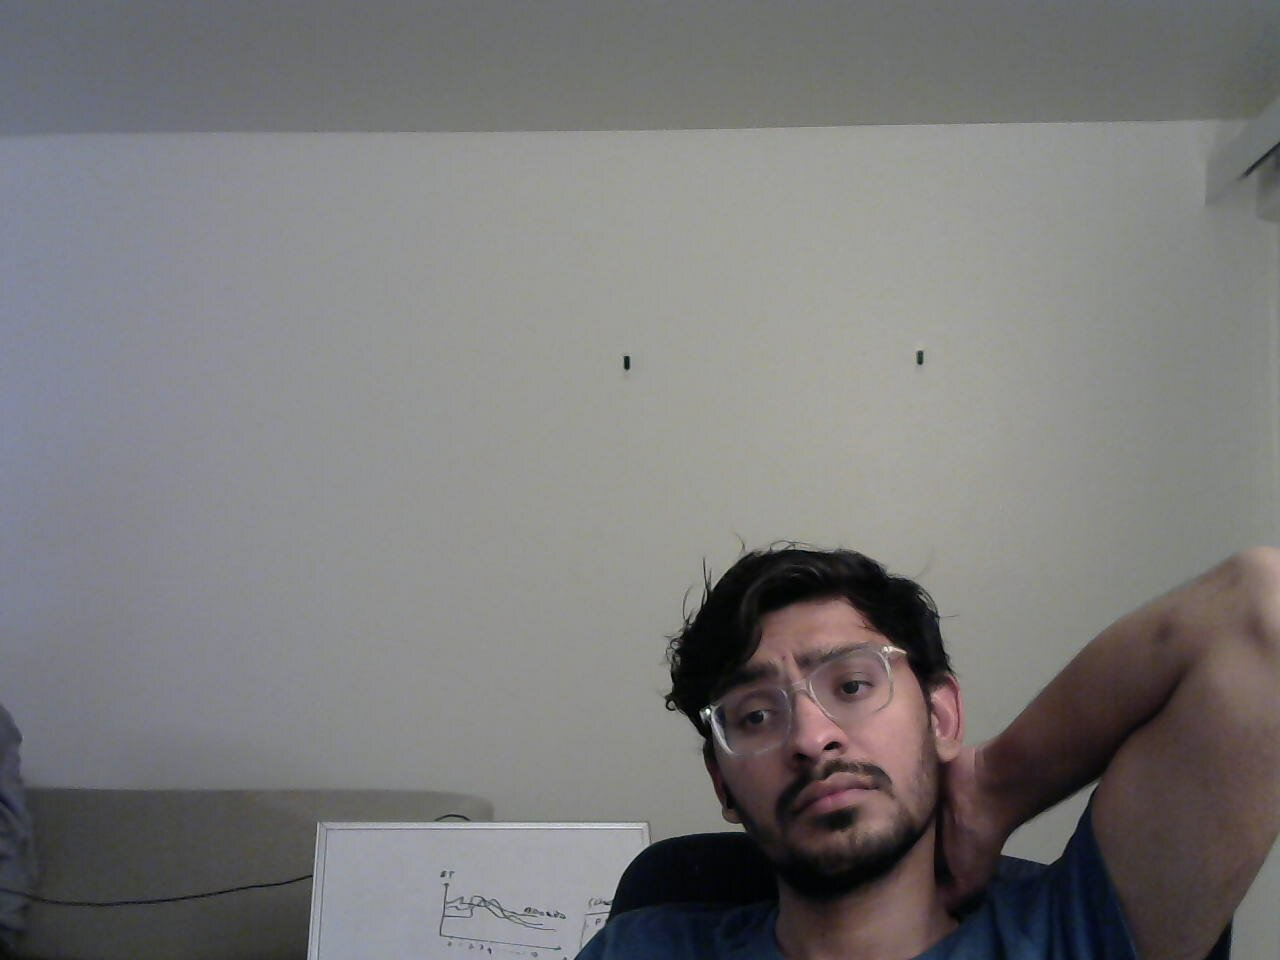
\includegraphics[scale=0.35]{figures/cheese.jpg}
				\caption{Cheese Output}
			\end{figure}


	\end{enumerate}




	\section{Question 3}
	\begin{enumerate}
		\item[] \Q [10 points] Using your verified Logitech C2xx camera on a DE1-SoC, Raspberry Pi or Jetson, verify
			that it can stream continuously to a raw image buffer for transformation and processing using any
			one of the below methods:
			\A
			\begin{enumerate}
				\item Update Package Index and Install Prerequisites: This step involves updating the package index on your Linux system and installing the minimal prerequisites required to compile OpenCV, such as cmake, g++, wget, and unzip.
				\item Download OpenCV Sources: The OpenCV source code is downloaded from its GitHub repository. The wget command is used to fetch the zip archive of the OpenCV source code designated by the 4.x version tag, which is then unpacked using unzip.
				\item Create a Build Directory: A separate build directory is created to keep the compilation process organized and separate from the source code.
				\item Configure the Build: The cmake command is used to configure the build environment. This step prepares the makefile based on the available source code and specified options.
				\item Compile OpenCV: The compilation process is initiated with the cmake --build . command. This step compiles the source code into executable binaries and libraries.
			\end{enumerate}


			\begin{lstlisting}[language=sh]
# Install minimal prerequisites (Ubuntu 18.04 as reference)
sudo apt update && sudo apt install -y cmake g++ wget unzip

# Download and unpack sources
wget -O opencv.zip https://github.com/opencv/opencv/archive/4.x.zip
unzip opencv.zip

# Create build directory
mkdir -p build && cd build

# Configure
cmake ../opencv-4.x

# Build
cmake --build .

# make 
make -j4

# make install
sudo make install
		\end{lstlisting}

			\begin{figure}[H]
				\centering
				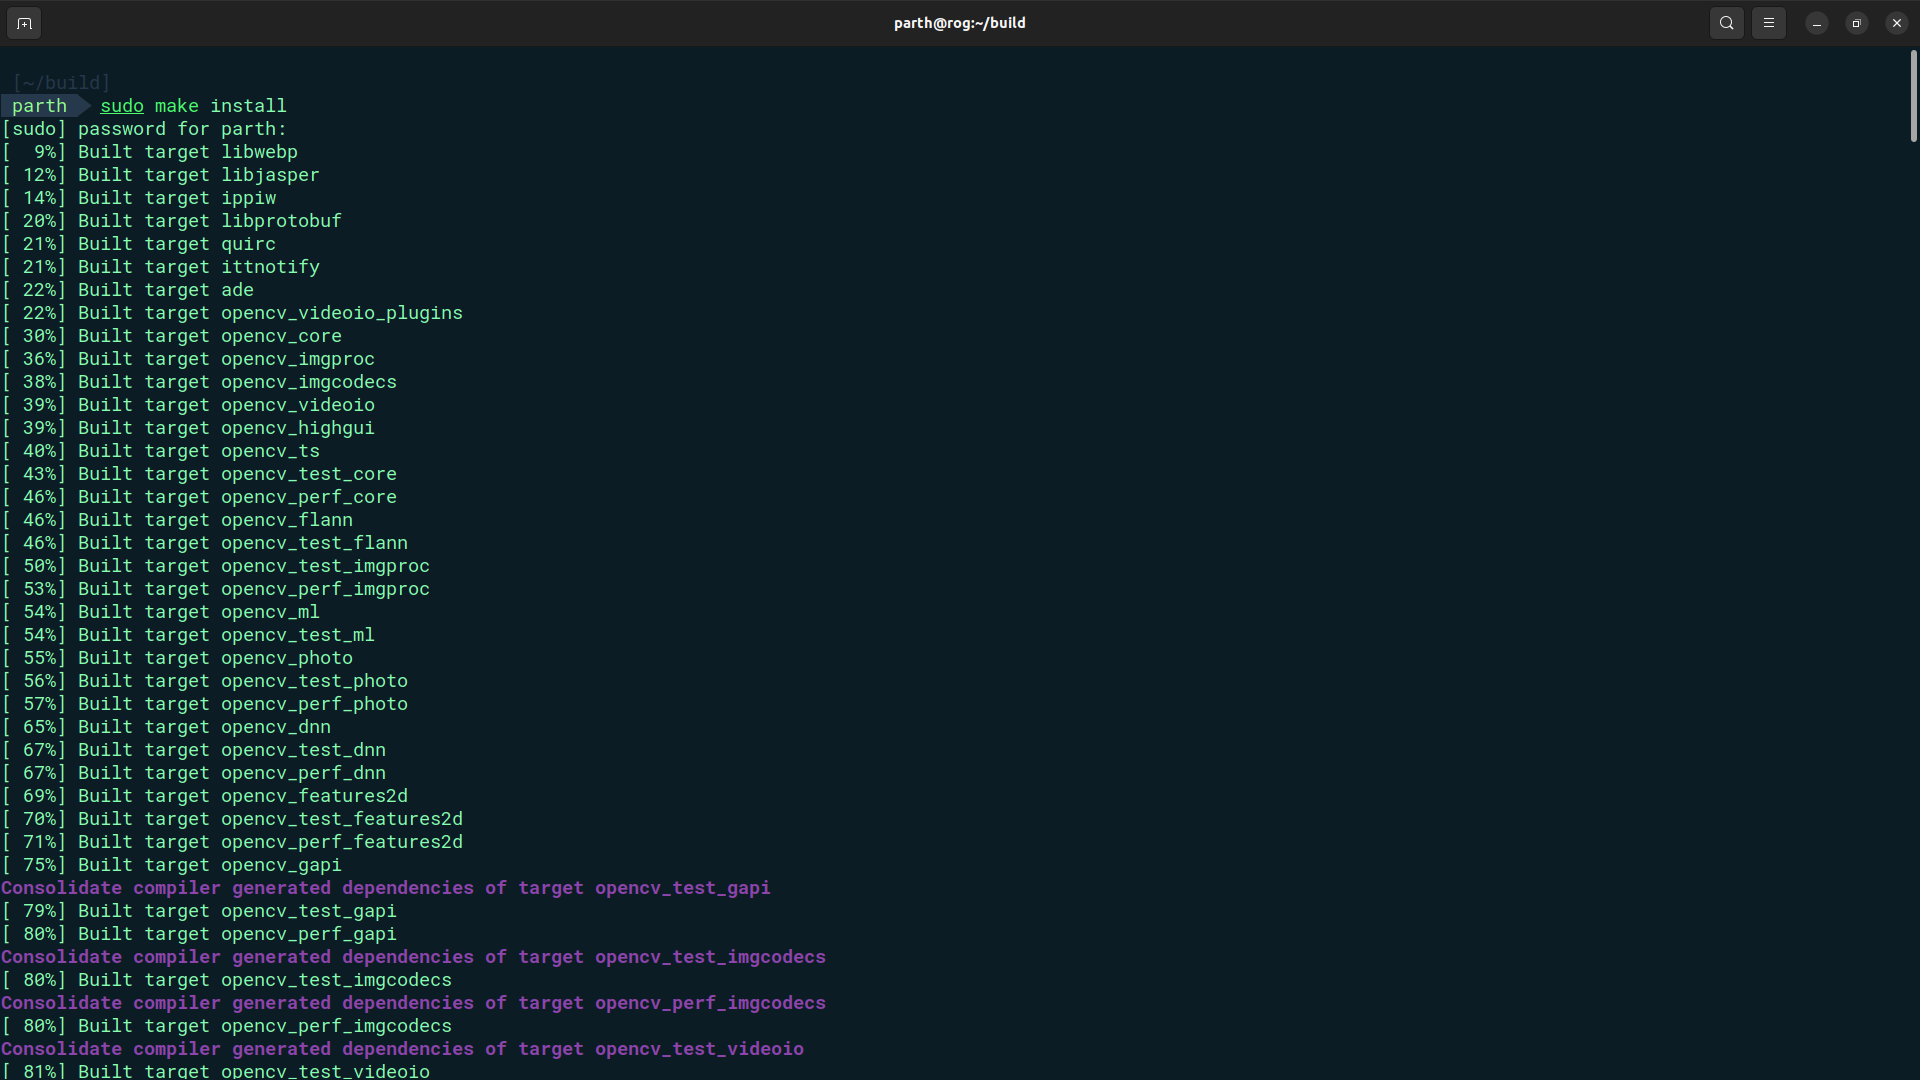
\includegraphics[scale=0.25]{figures/build1.png}
				\caption{Build 1}
			\end{figure}
			\begin{figure}[H]
				\centering
				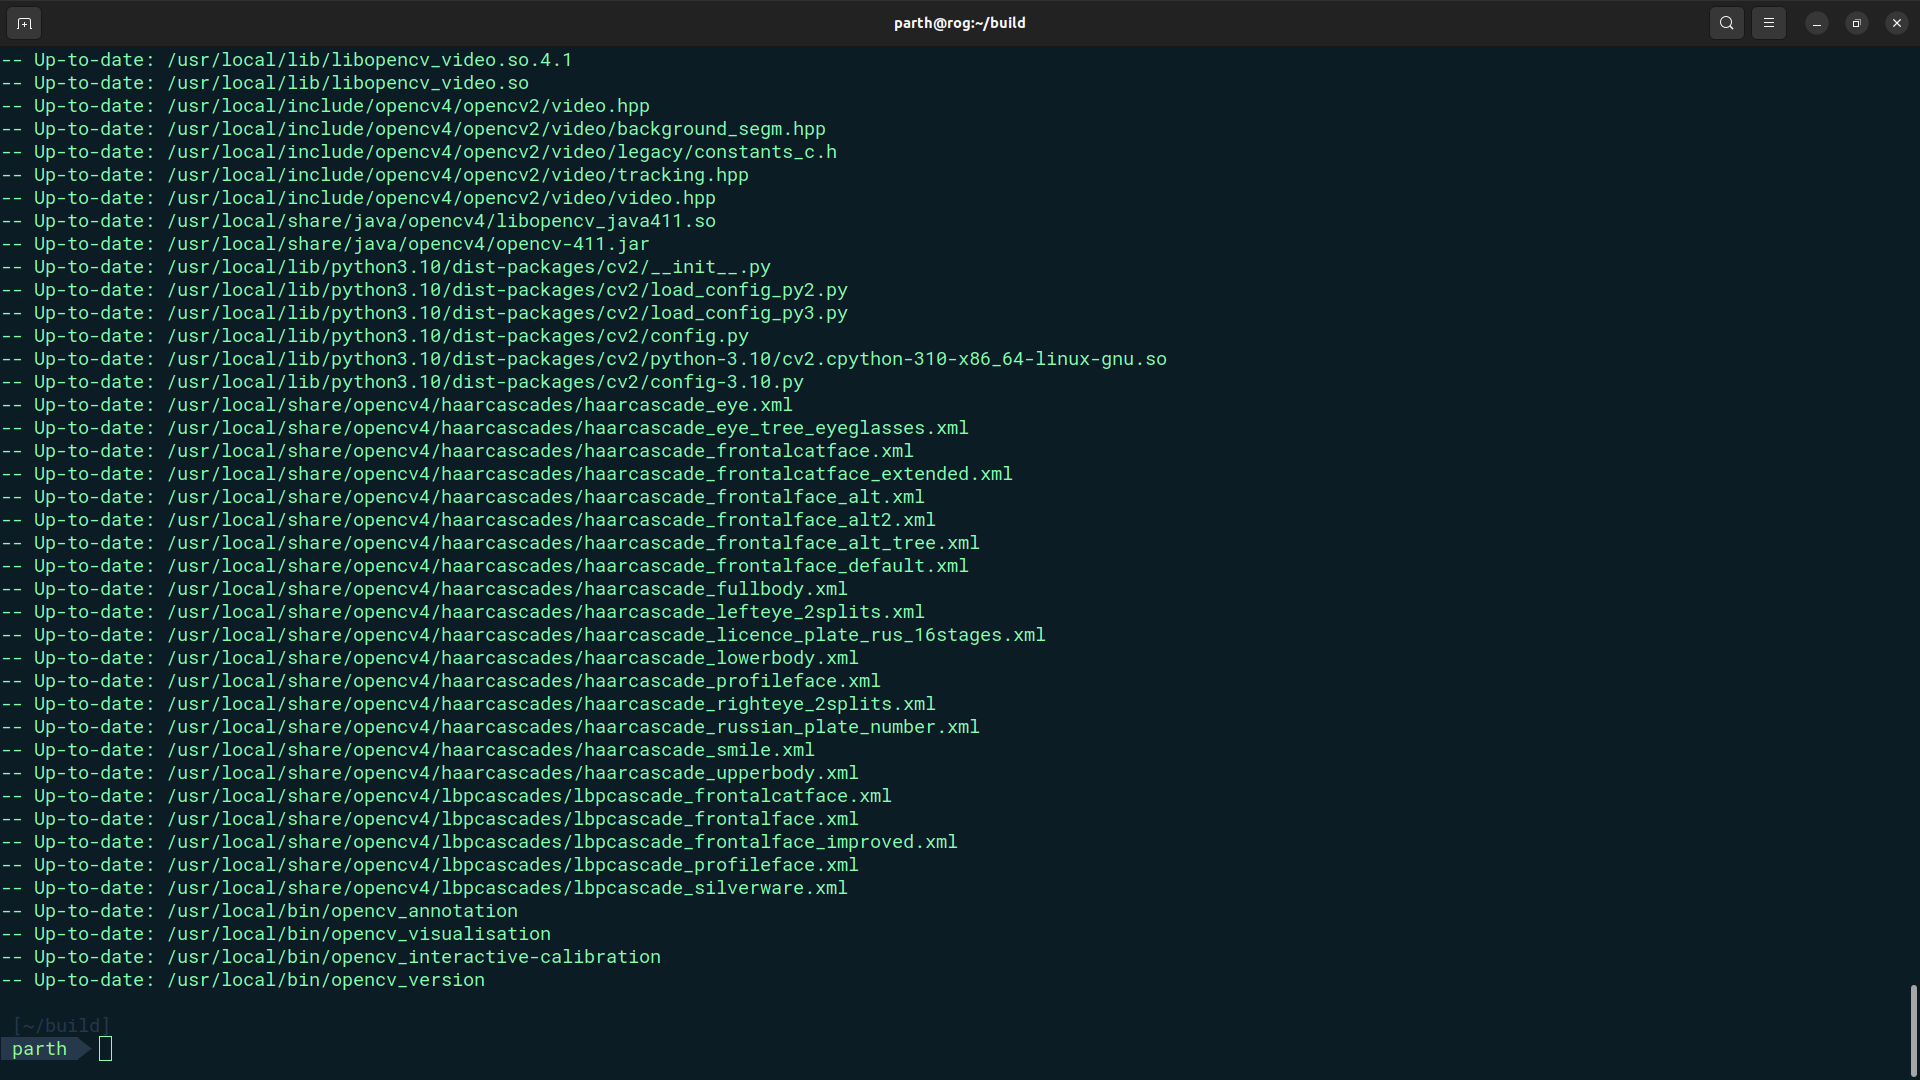
\includegraphics[scale=0.25]{figures/build2.png}
				\caption{Build 2}
			\end{figure}
			\begin{figure}[H]
				\centering
				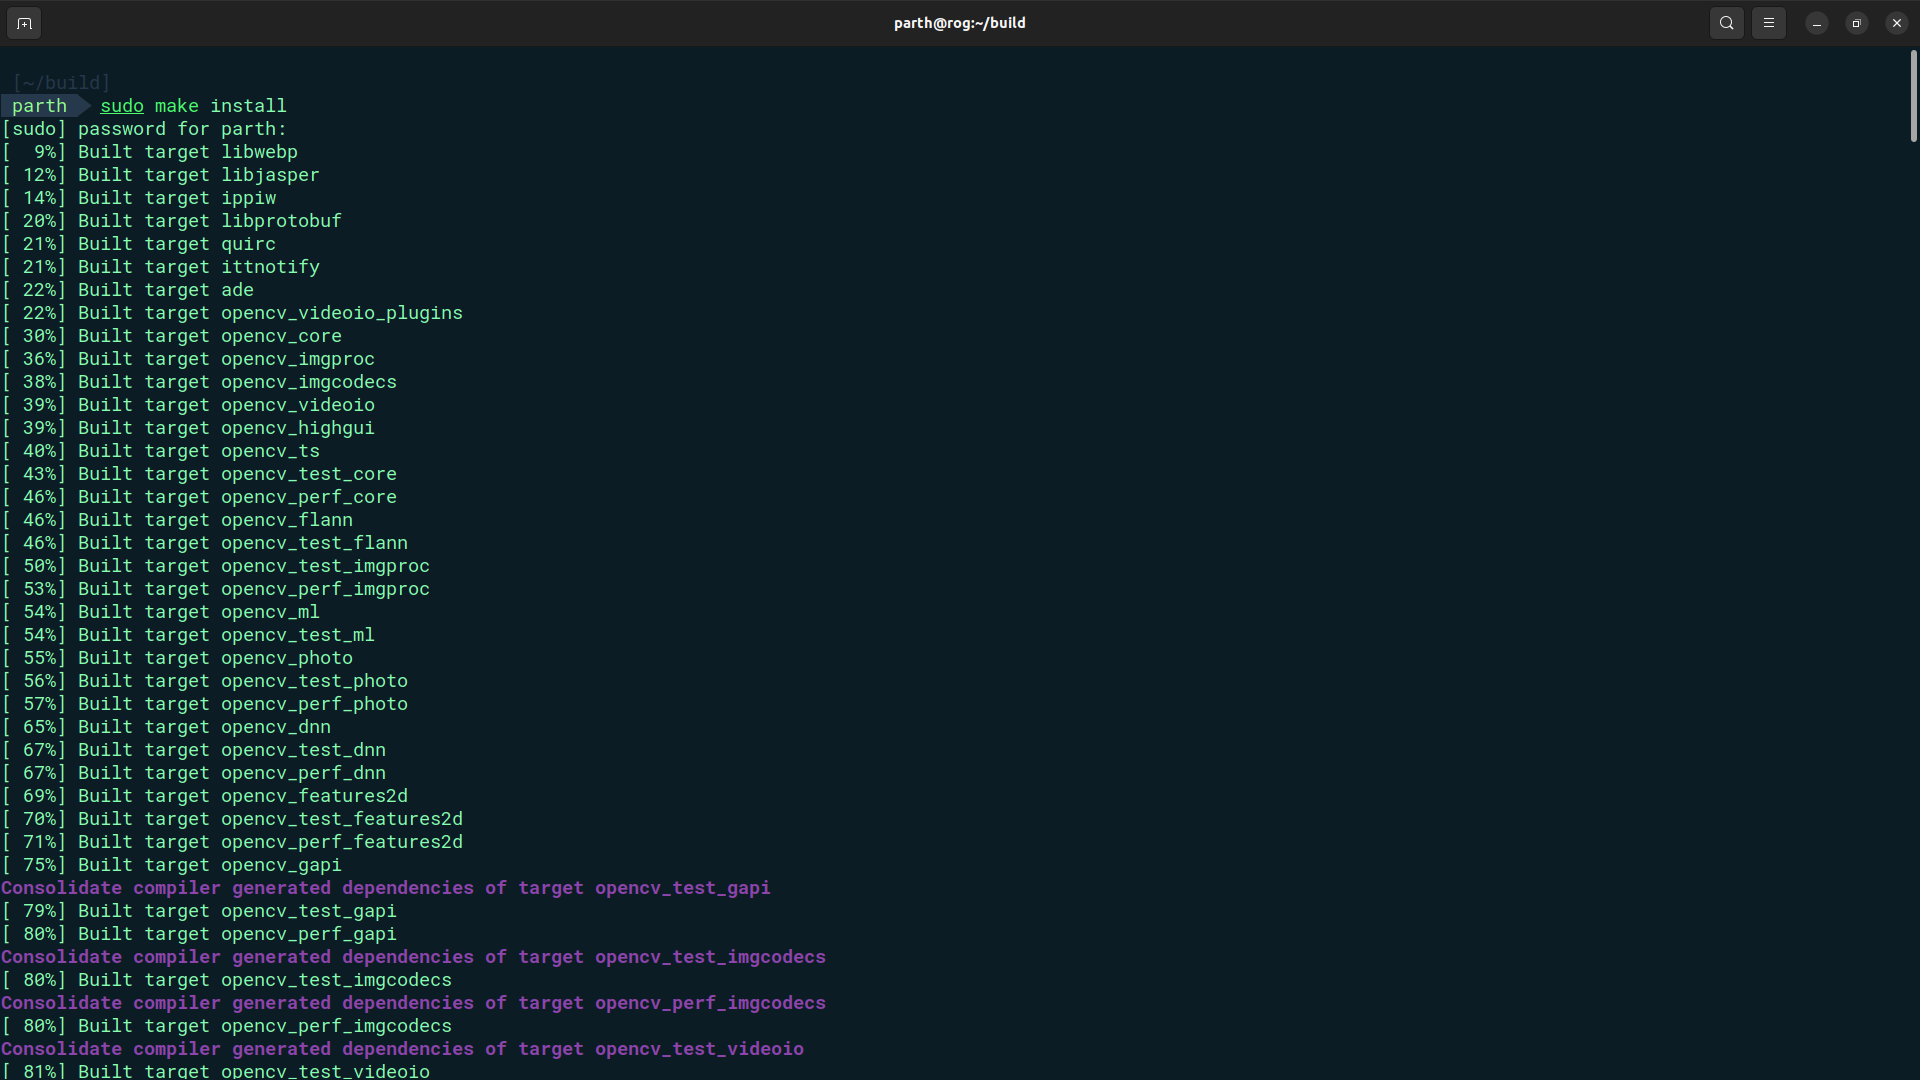
\includegraphics[scale=0.25]{figures/build3.png}
				\caption{Build 3}
			\end{figure}
			\begin{figure}[H]
				\centering
				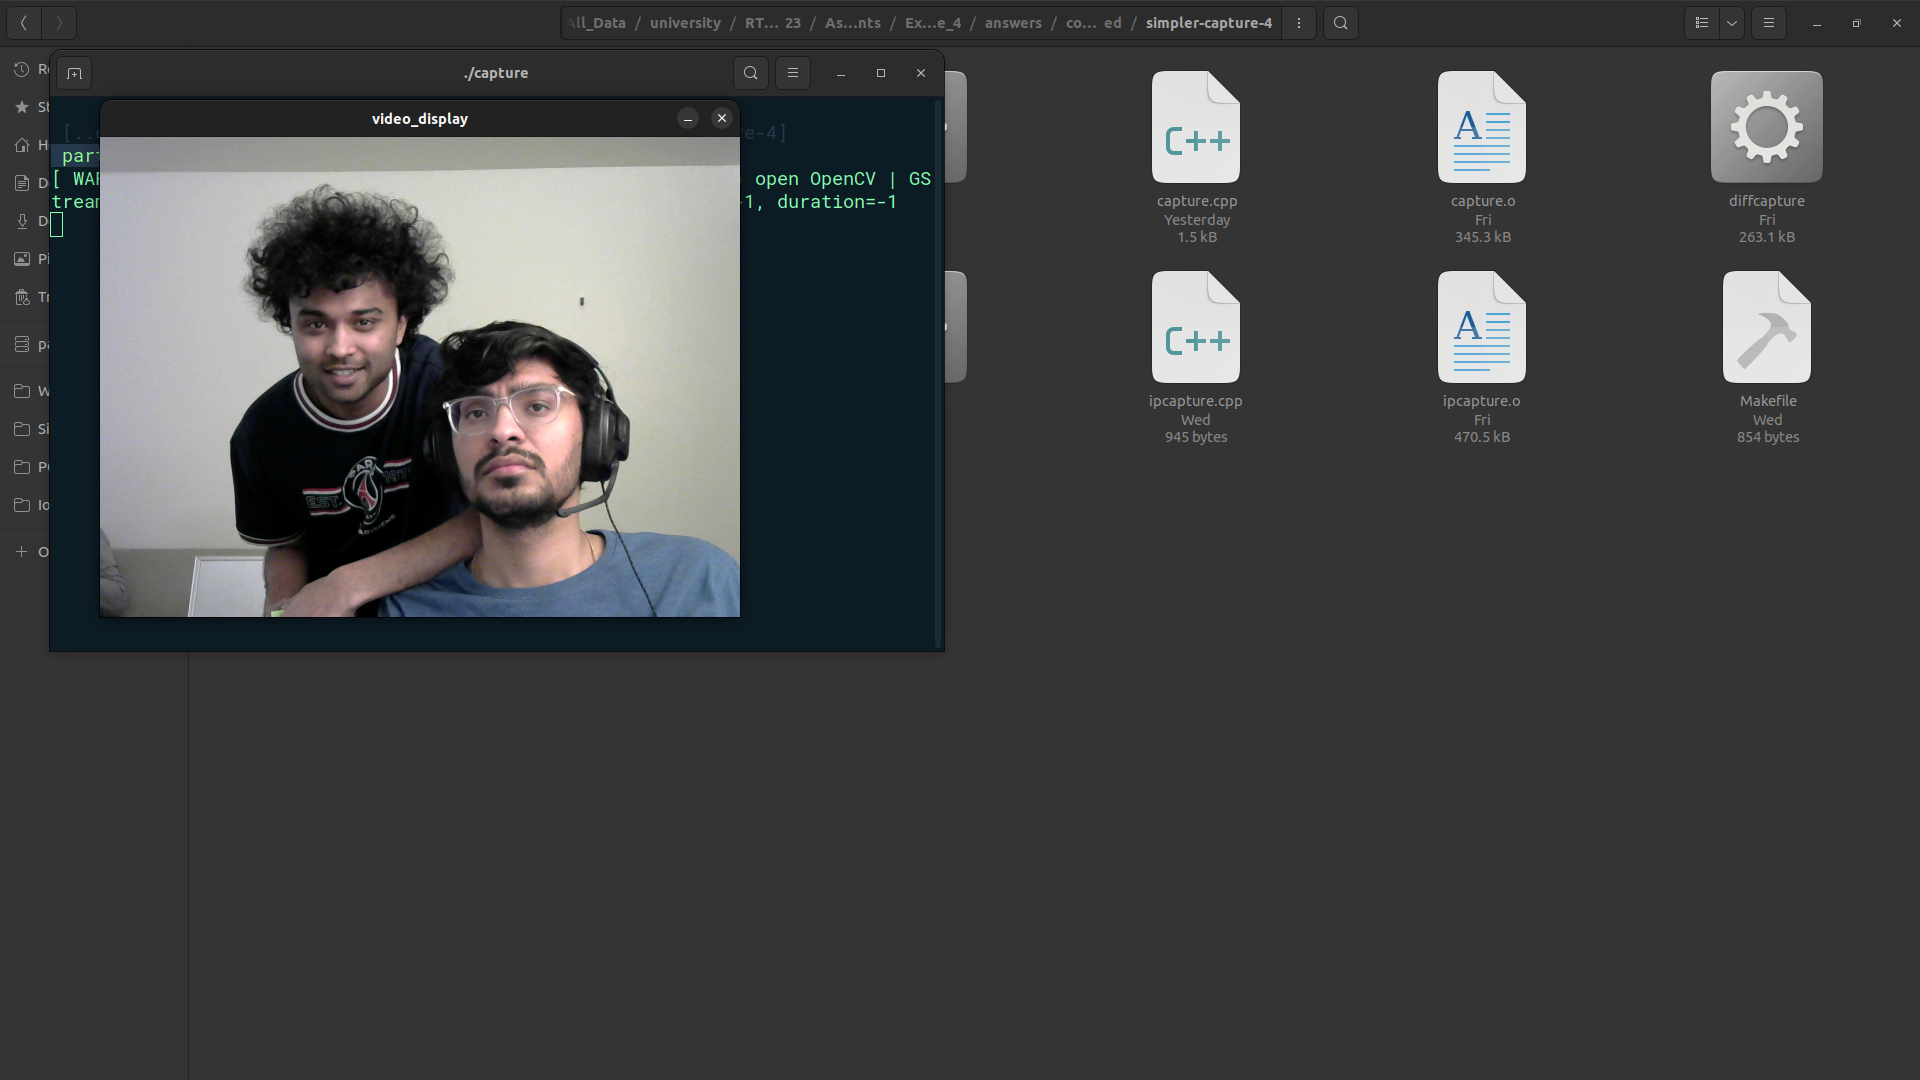
\includegraphics[scale=0.25]{figures/continuous_capture.png}
				\caption{Build 4}
			\end{figure}

			\begin{enumerate}
				\item VideoCapture cam0(0);: Creates an object cam0 for capturing video from the camera. The parameter (0) specifies the first camera device. This class provides a way to interact with the video capturing functionality of OpenCV.
				\item namedWindow\("video_display"\);: Creates a window named "video\_display" for displaying the video. This function is part of the High-level GUI module.
				\item cam0.isOpened(): Checks if the video capture device has been successfully initialized.
				\item exit(SYSTEM\_ERROR);: Exits the program with a system-defined error status if the camera cannot be opened.
				\item cam0.set\(CAP\_PROP\_FRAME\_WIDTH, 640\); and cam0.set\(CAP\_PROP\_FRAME\_HEIGHT, 480\);: Sets the properties of the capture device, specifically the frame width and height to 640x480 pixels. CAP\_PROP\_FRAME\_WIDTH and CAP\_PROP\_FRAME\_HEIGHT are predefined constants that specify which property to set.
				\item Mat frame\(640, 480, \);: Defines a matrix (Mat) object named frame to store individual frames captured from the camera. The constructor parameters typically include the dimensions and the type of the matrix, but here it seems to be a typo or an incomplete line of code, as the type is missing.
				\item cam0.read\(frame\);: Captures the next frame from the video capture device and stores it in frame. This method returns false if no frames have been captured.
				\item imshow\("video\_display", frame\);: Displays the frame in the window named "video\_display". This function is called within the loop to continuously update the window with new frames from the camera.
				\item waitKey(10): Waits for a key event for a brief period (10 milliseconds). This function is essential for the GUI to process events and update the window. The return value is stored in winInput.
				\item if ((winInput = waitKey(10)) == ESCAPE\_KEY): Checks if the ESC key \(ASCII value 27\) has been pressed. If so, it breaks out of the loop, ending the video capture.
				\item destroyWindow\("video_display"\);: Closes the window named "video\_display" before the program exits.
			\end{enumerate}
		
	\end{enumerate}

	\pagebreak
	\section{Question 4}
	\begin{enumerate}
		\item[] \Q [15 points] Review POSIX-examples and especially POSIX\_MQ\_LOOP and build the code
			related to POSIX message queues and run them to learn about basic use.
			\A
			\begin{enumerate}
				\item 
			\end{enumerate}
			
				\textbf{Canny}
				Here's an explanation of the provided Code
				\begin{itemize}
					\item Mat variables canny\_frame, timg\_gray, timg\_grad, and frame are declared to store
					image data.
					\item Integer variables lowThreshold, max\_lowThreshold, ratio, and kernel\_size are declared
					for Canny edge detection parameters.
				\end{itemize}


CannyThreshold Function:
\begin{itemize}
	\item This function is used to perform Canny edge detection on the captured frame.
	\item It converts the frame to grayscale using cvtColor().
	\item Noise reduction is applied using blur().
	\item Canny edge detection is performed using Canny().
	\item The result is displayed in the window\_name window using imshow().
\end{itemize}

Main Function:\
\begin{itemize}
	\item Video capture object cam0 is initialized for the default camera (index 0).
	\item A window named "video\_display" is created for displaying the captured video frames.
	\item The frame size is set to 640x480 pixels using cam0.set().
	\item Within a while loop:
	\item Frames are continuously captured from the camera using cam0.read().
	\item The captured frame is displayed in the "video\_display" window using imshow().
	\item The Canny edge detection trackbar is created and CannyThreshold function is called to
	apply edge detection on the frame.
	\item The program exits the loop if the escape key (ESC) is pressed.
\end{itemize}

This code captures video frames from the camera, performs Canny edge detection, and

\textbf{Cannycam}
\begin{figure}[H]
	\centering
	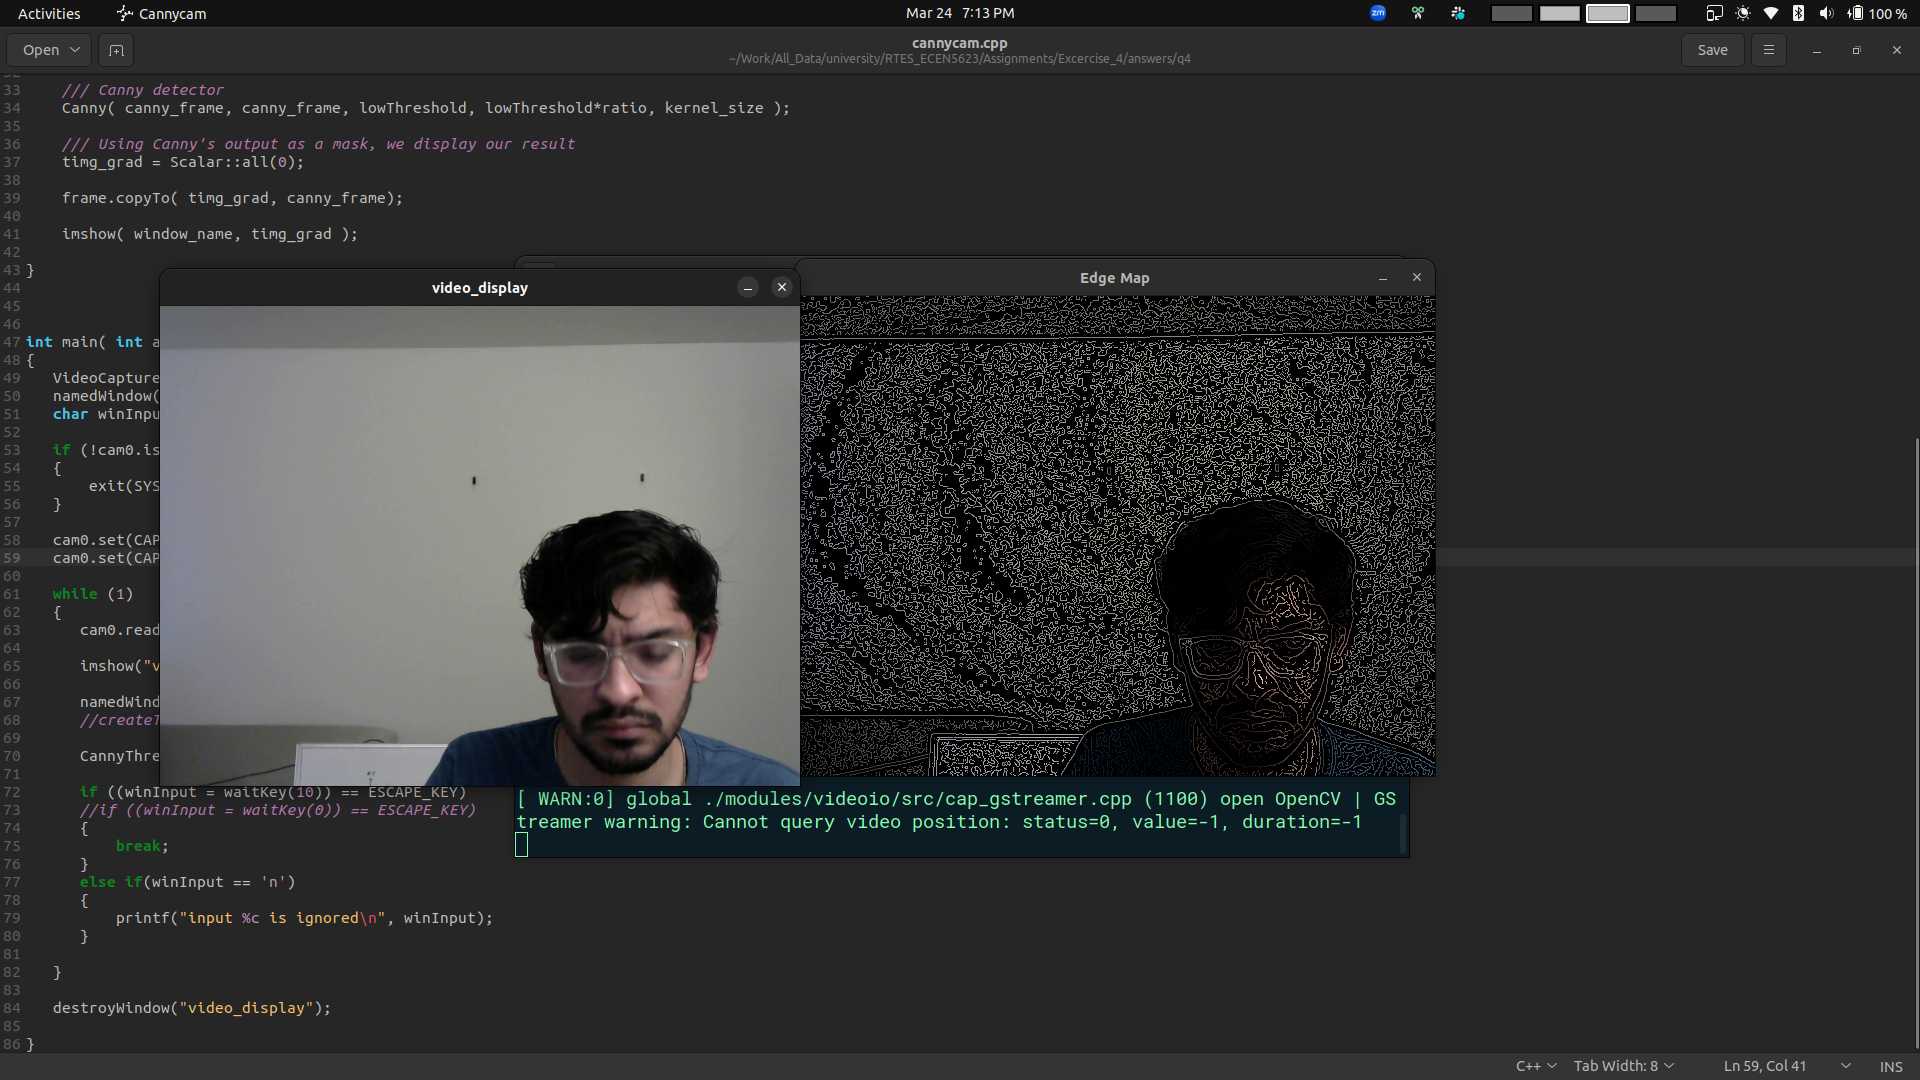
\includegraphics[scale=0.25]{figures/canny.png}
	\caption{Canny}
\end{figure}
\textbf{Cannycam top}
\begin{figure}[H]
	\centering
	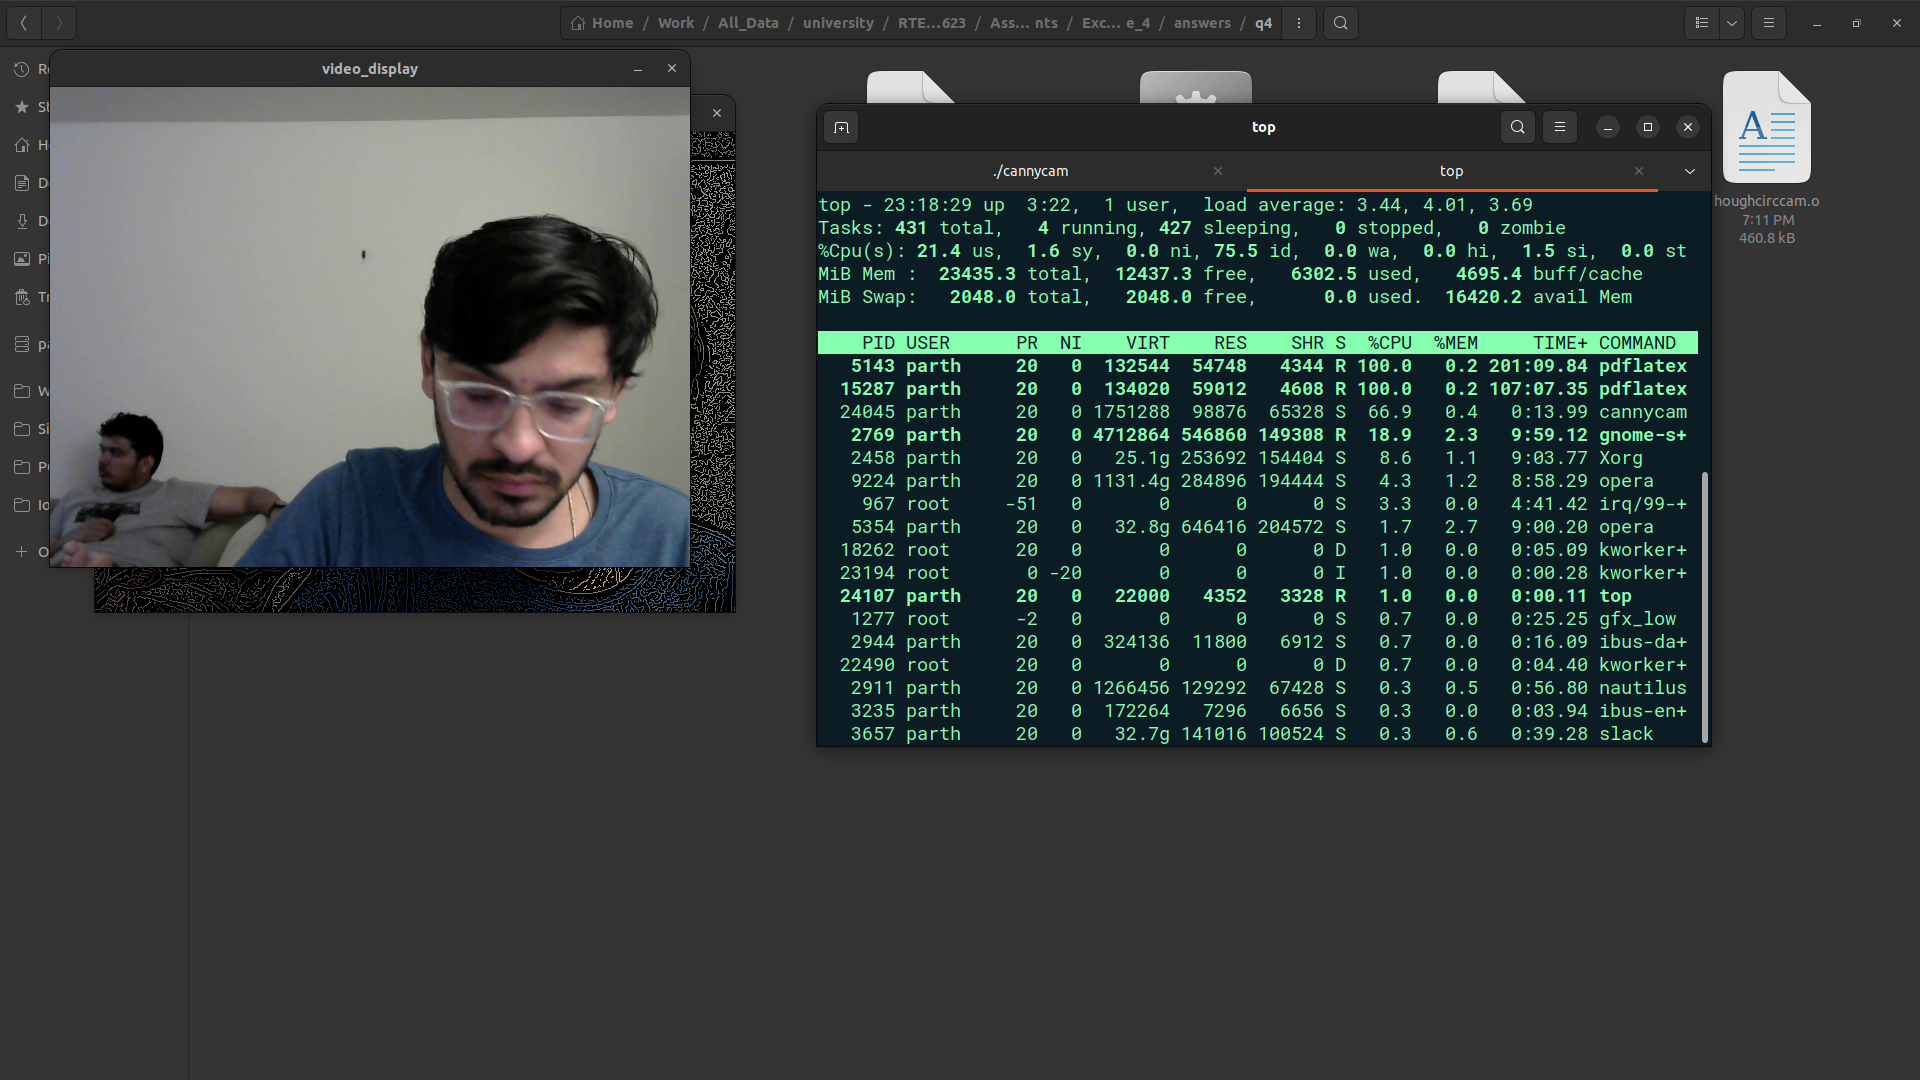
\includegraphics[scale=0.25]{figures/canny_htop.png}
	\caption{Canny Top}
\end{figure}

Here's an explanation of the provided code
\begin{itemize}
	\item Mat variables dst, cdst, and cdstP are declared to store images.
	default\_file and filename are declared to store the default image file path and the actual
	image file path, respectively.
	src is declared to store the loaded image.
	\item Image Loading:
	imread() function is used to load an image from the specified file path (filename) in
	grayscale mode (IMREAD\_GRAYSCALE).
	\item Edge Detection (Canny):
	Canny() function is applied to detect edges in the loaded image (src). The detected
	edges are stored in the dst matrix.
	\item Color Conversion:
	cvtColor() function converts the grayscale edge image (dst) to a BGR (Blue-Green-Red)
	color image (cdst) for visualization.
	\item Standard Hough Line Transform:
	HoughLines() function detects lines in the edge image (dst) using the Standard Hough
	\item Drawing Detected Lines:
	For each detected line, line() function draws a line on the output image (cdst) using the
	line parameters (rho and theta).
	Probabilistic Hough Line Transform:
	HoughLinesP() function detects lines in the edge image (dst) using the Probabilistic
	Hough Line Transform. Detected lines are stored in the linesP vector.
	\item Drawing Probabilistic Detected Lines:
	For each detected line, line() function draws a line on the output image (cdstP) using the
	line parameters (x1, y1, x2, y2). Additionally, lines are drawn on the original image (src)
	to visualize the detected lines.
	\item Displaying Results:
	imshow() function displays the original image (src) and the image with detected lines
	(cdstP) in separate windows.
	This code loads an image, performs edge detection using the Canny algorithm, detects lines in
	the edge image using both the Standard Hough Line Transform and the Probabilistic Hough
	Line Transform, and visualizes the detected lines on the original image. Finally, it displays the
	results in separate windows and waits for a key press before exiting.	

\end{itemize}

\textbf{Hough Line Transform}


The following changes have been made to the houghline.cpp code to make it work with\\
continuous video input in houghlinecam.cpp:
\begin{itemize}
	\item Video Capture: The houghlinecam.cpp code includes the opencv2/videoio.hpp header
	file to access the video capture functionality. It creates a VideoCapture object cam0 to
	read frames from the default camera (index 0).
	\item Continuous Video Processing Loop: The code enters a continuous loop where it reads
	frames from the camera using cam0.read(frame), displays the frame in the
	"video\_display" window using imshow("video\_display", frame), performs edge detection using the Canny algorithm, copies the edges to the output images (cdst and cdstP), and
	calls the HoughLinePTransform() function to detect and draw lines.
	\item Keyboard Input Handling: The loop checks for keyboard input using waitKey(10), which
	waits for 10 milliseconds for a key press. If the ESC key is pressed, the loop breaks and
	the program exits. If the 'n' key is pressed, it prints a message indicating that the input is
	ignored.
	\item Hough Line Probabilistic Transform Function: The HoughLinePTransform() function is
	defined to encapsulate the Probabilistic Hough Line Transform operation. This function
	performs the transform on the dst image (containing the edges), draws the detected lines
	on the cdstP and src (original frame) images using the line function, and displays the
	result in a window named "Prob HL Transform".
	\item Window Destruction: After the continuous loop exits, the "video\_display" window is
\end{itemize}


closed using the destroyWindow function.
\begin{figure}[H]
	\centering
	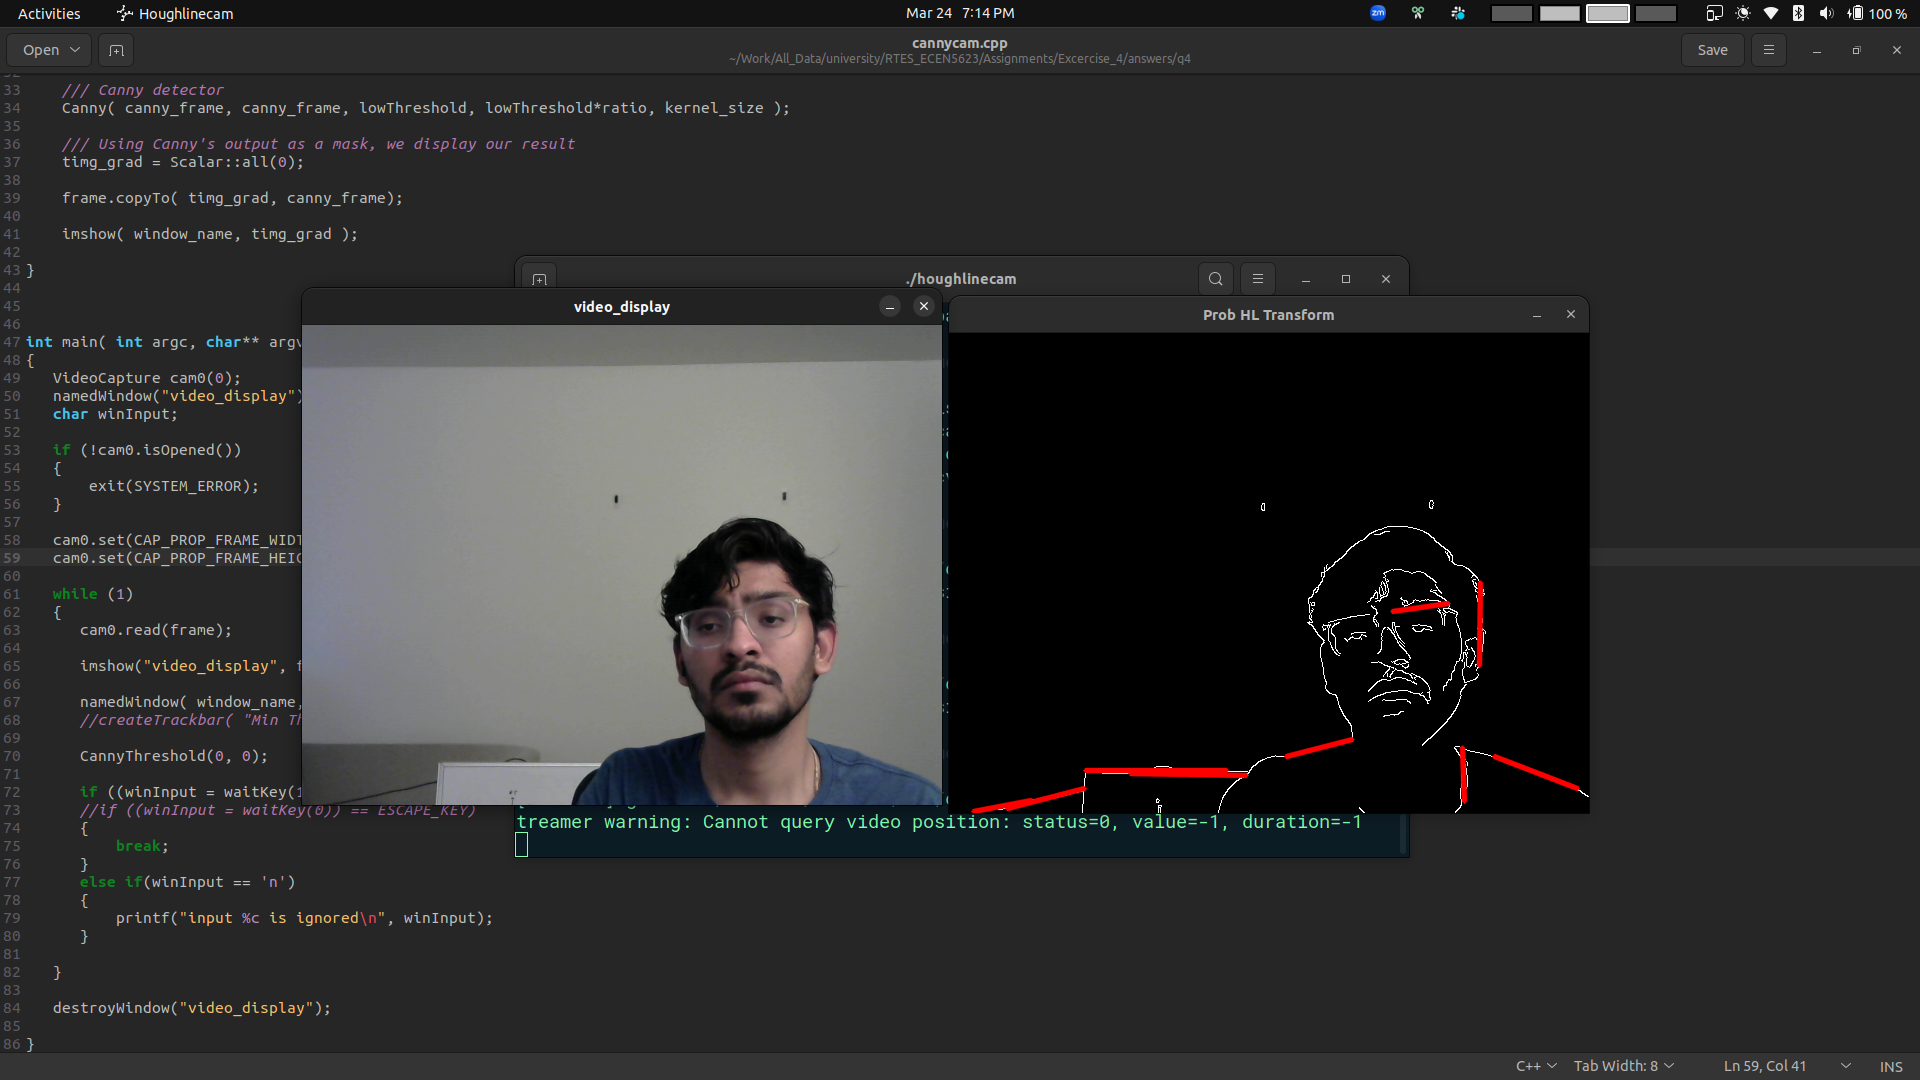
\includegraphics[scale=0.25]{figures/houghline.png}
	\caption{Hough Line}
\end{figure}

\textbf{Hough Line Transform top}
\begin{figure}[H]
	\centering
	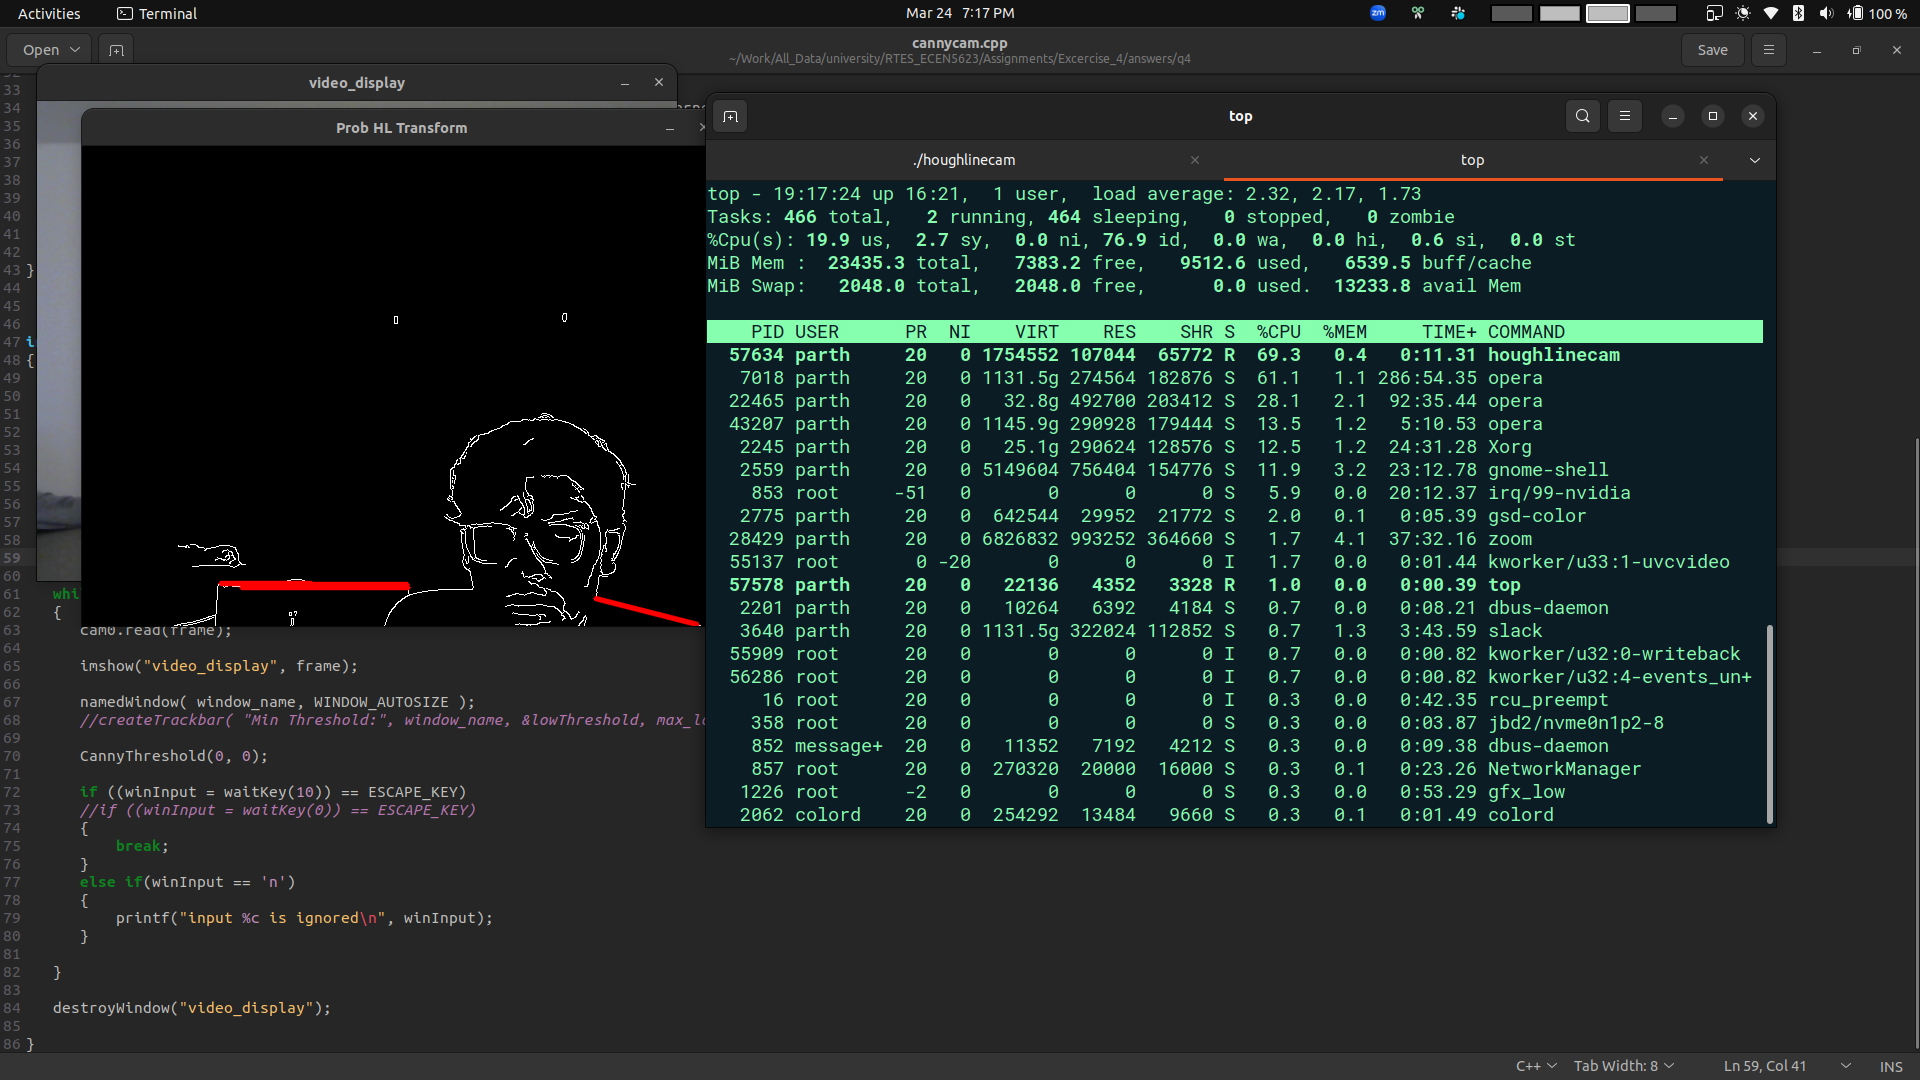
\includegraphics[scale=0.25]{figures/htop.png}
	\caption{Hough Line Top}
\end{figure}




\textbf{Hough Circle Transform}
Here's an explanation of the provided code
\begin{itemize}
	\item Image Loading:
	This code (main() function) loads an image specified by the user or uses a default image
	("../data/smarties.png") if no argument is provided.
	\item Image Processing:
	\item The loaded image (src) is directly converted to grayscale using cvtColor() and then
	median blur is applied to the grayscale image.
	\item Circle Detection:
	Detect circles in the processed grayscale image using the Hough Circle Transform
	(HoughCircles() function).
	\item Circle Drawing:
	After detecting circles, draw circles on the original color image (src) using the circle()
	function.
	Image Display:
	Finally, display the image with detected circles using imshow() and wait for a key press
	using waitKey() before exiting.
\end{itemize}



\begin{figure}[H]
	\centering
	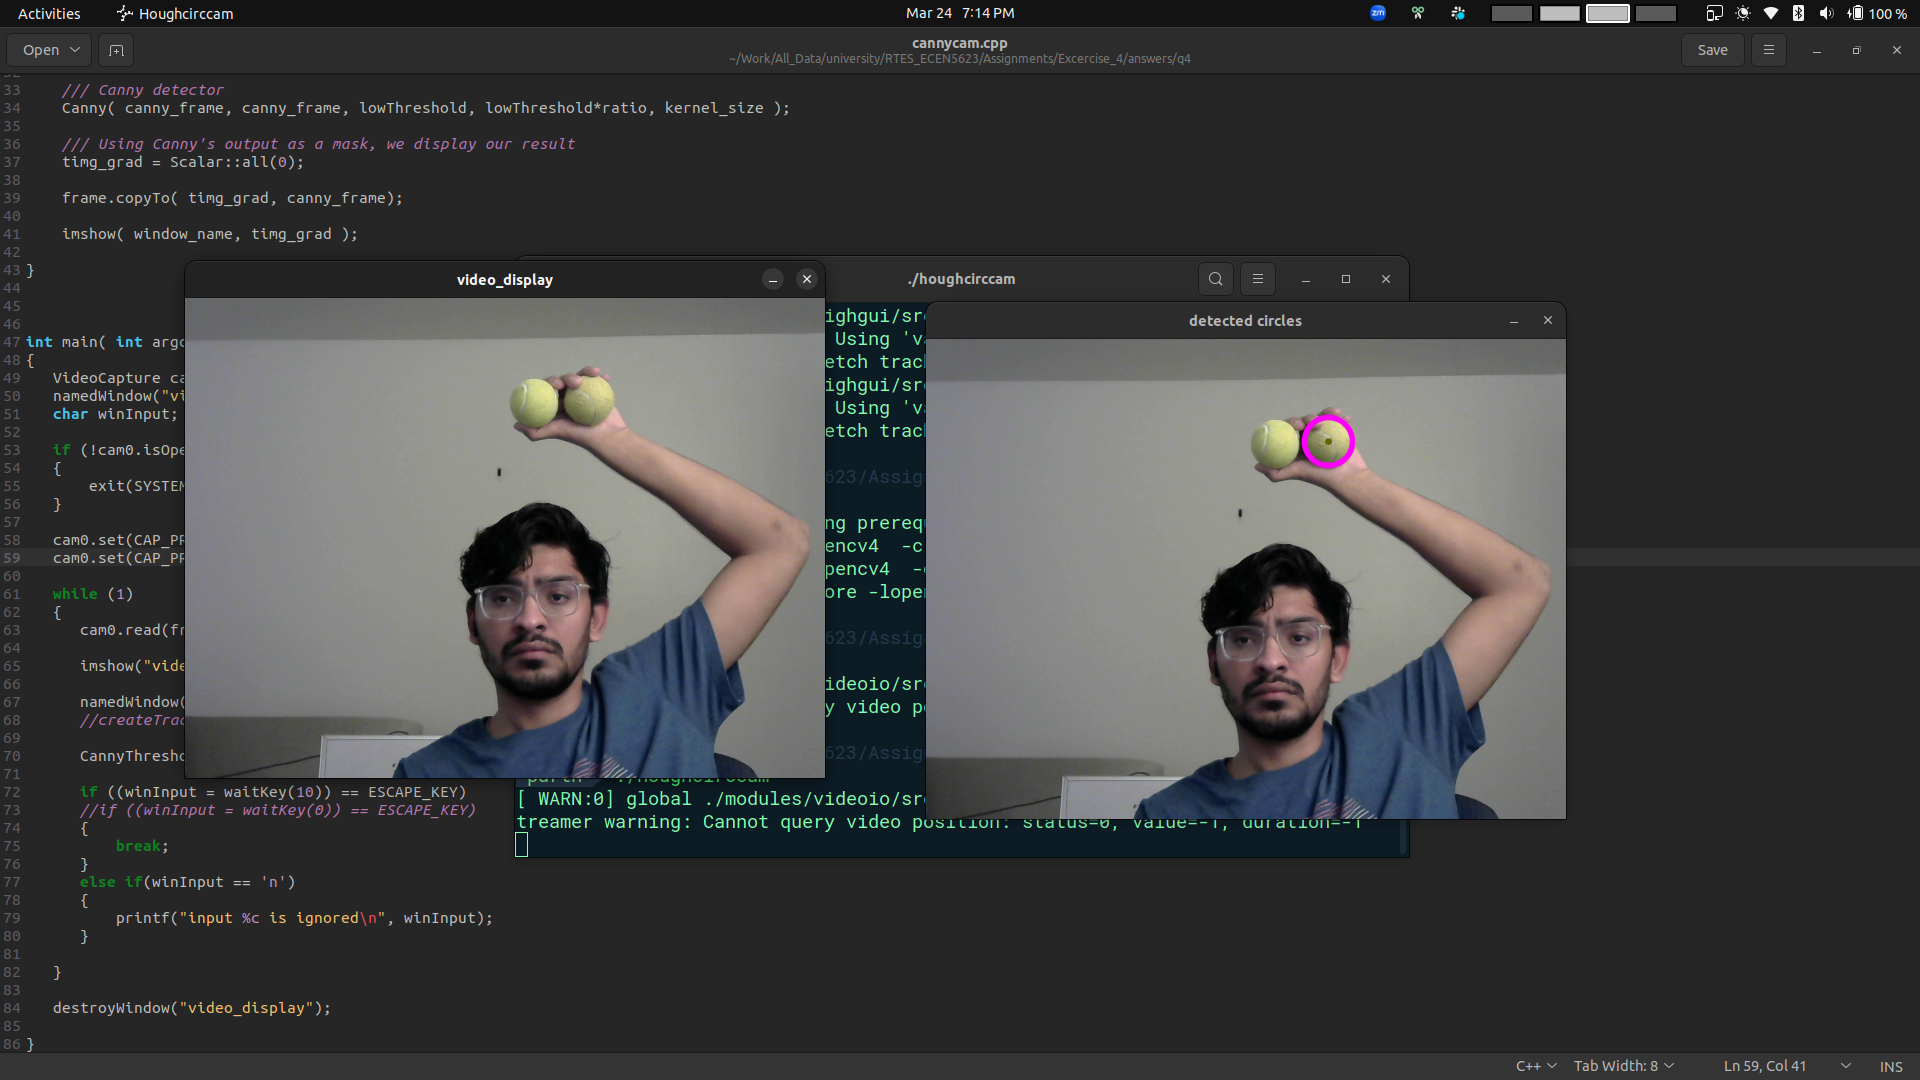
\includegraphics[scale=0.25]{figures/houghcircle.png}
	\caption{Hough Circle}
\end{figure}

\textbf{Hough Circle Transform top}
\begin{figure}[H]
	\centering
	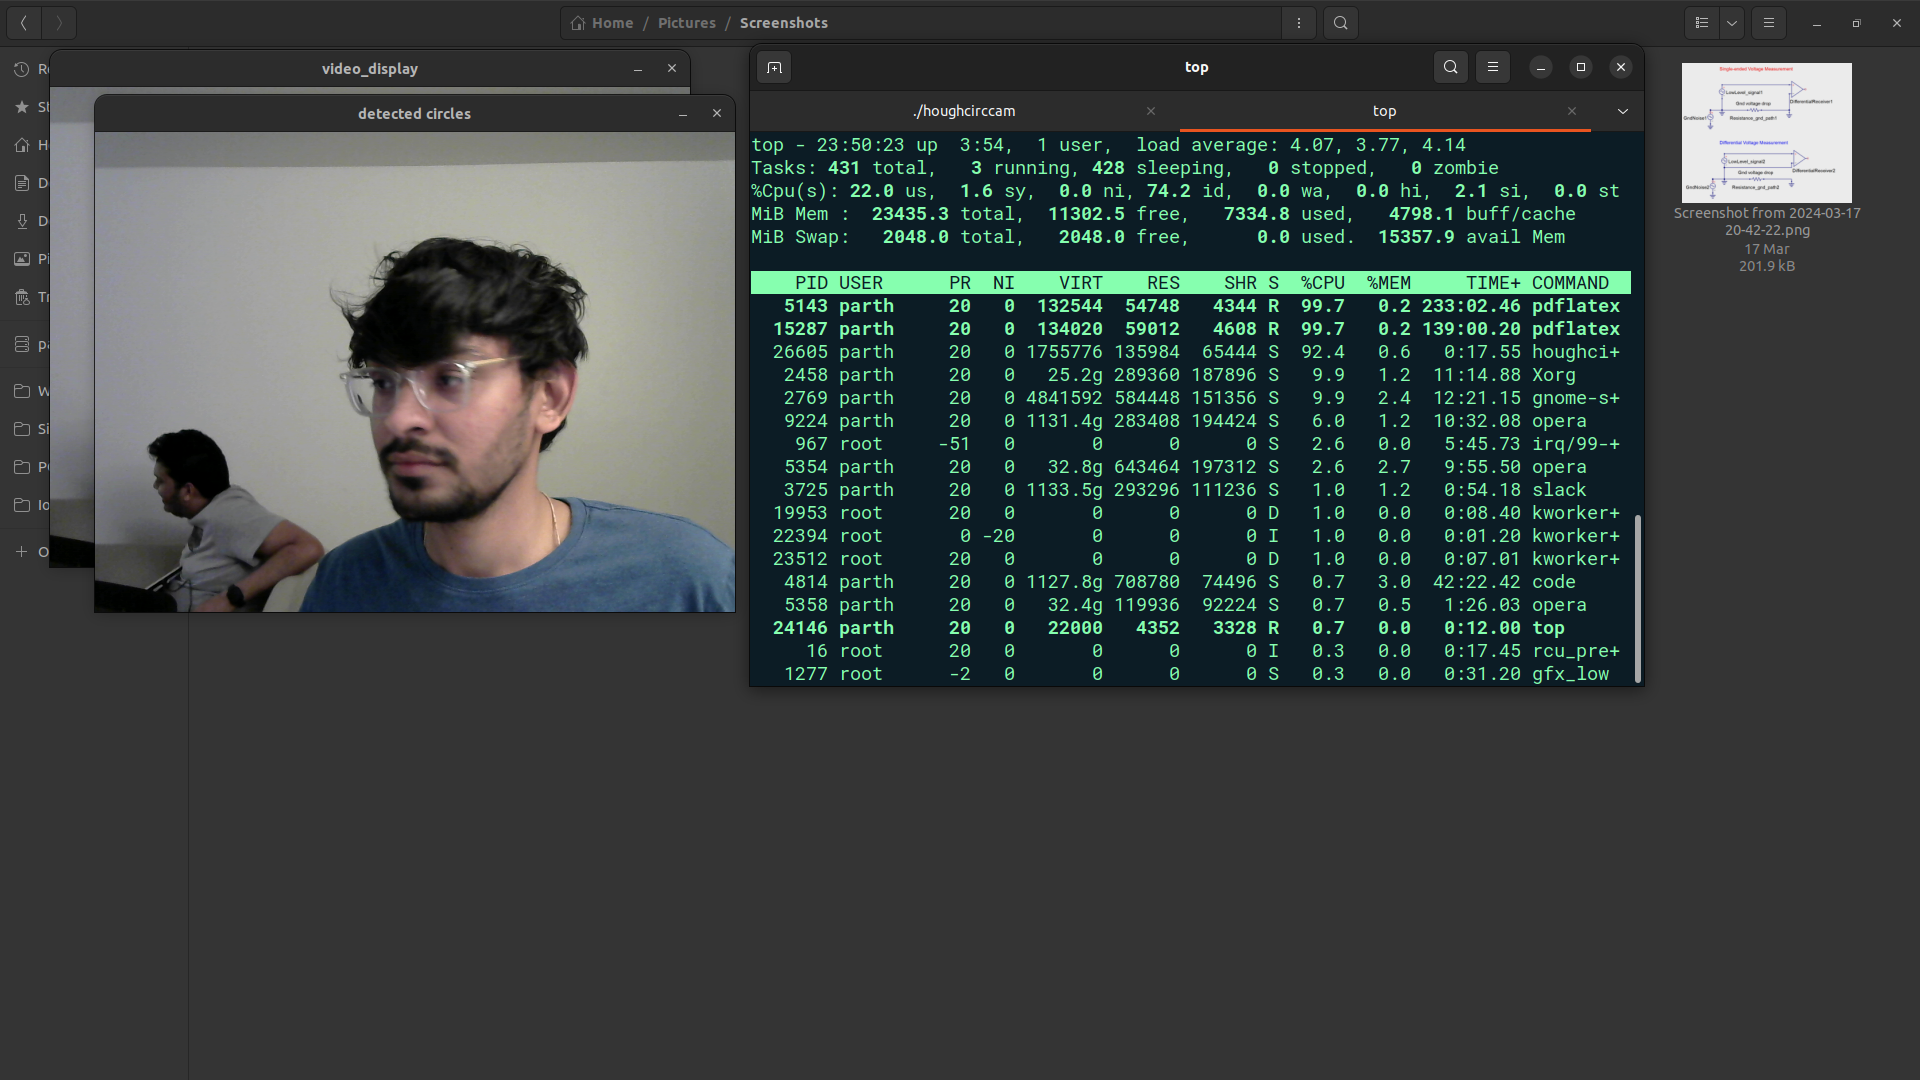
\includegraphics[scale=0.25]{figures/hc_htop.png}
	\caption{Hough Circle top}
\end{figure}			

	\end{enumerate}

	\section{Question 5}
	\begin{enumerate}
		\item[] \Q Using a Logitech C2xx, choose 3 real-time interactive transformations to compare in terms of
			average frame rate at a given resolution for a range of at least 3 resolutions in a common aspect
			ratio (e.g. 4:3 for 1280x960, 640x480, 320x240, 160x120, 80x60) by adding time-stamps (there
			should be a logging thread) to analyze the potential throughput. You should then get at least 9
			separate datasets running 1 transformation at a time. Based on average analysis, pick a
			reasonable soft real-time deadline \(e.g. if average frame rate is 12 Hz, choose a deadline of 100
			milliseconds to provide some margin\) and convert the processing to SCHED\_FIFO and
			determine if you can meet deadlines with predictability and measure statistical jitter in the frame
			rate relative to your deadline for both the default scheduler and SCHED\_FIFO in each case.
			\A

			\begin{enumerate}
				\item Design Concepts (Flow Chart or Diagram)
				      \begin{itemize}
					      \item Flow Chart/Diagram Creation:
					            \begin{figure}[H]
						            \centering
						            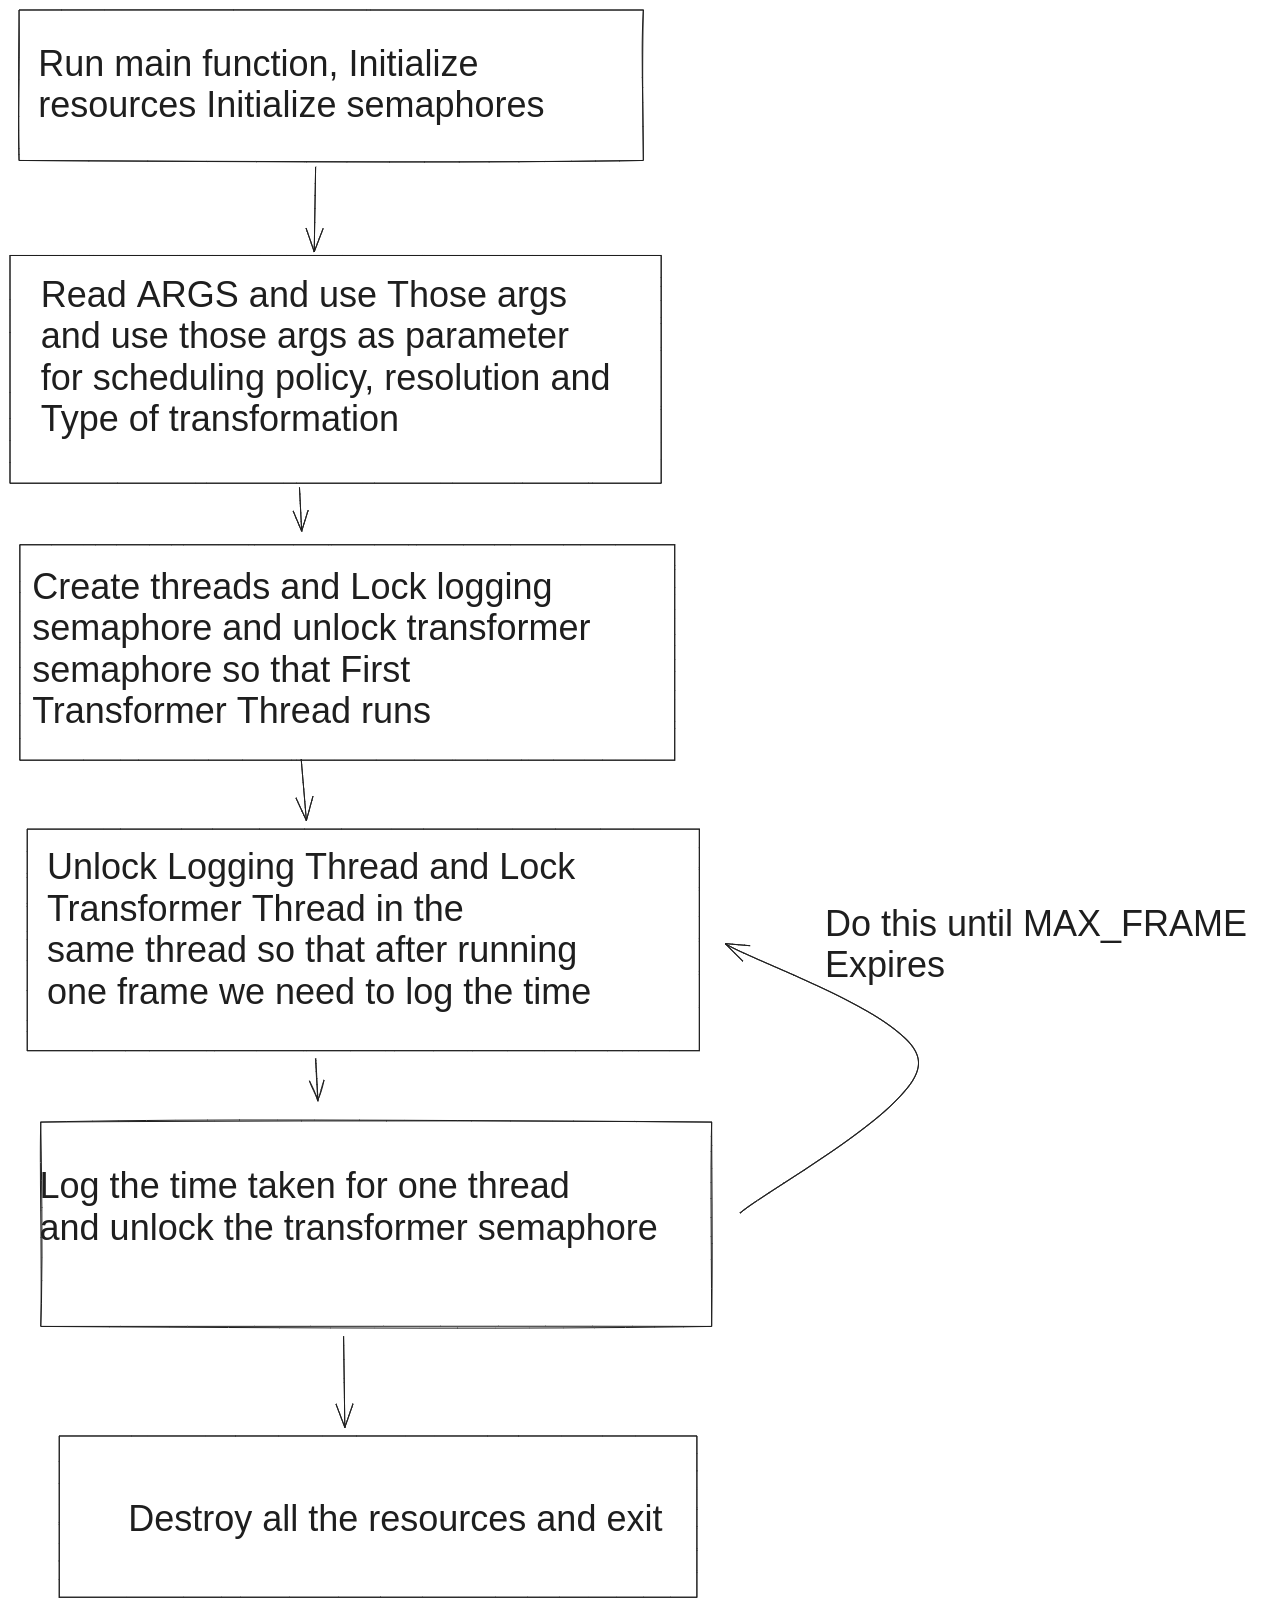
\includegraphics[scale=0.40]{figures/flowchard.png}
						            \caption{Flowchart}
					            \end{figure}
					      \item Components to Include:
					            \begin{itemize}
						            \item Video Capture and Processing: Utilizes OpenCV to capture video frames from a camera, apply image processing transformations (Canny edge detection, Hough Line and Circle Transforms), and display the transformed images.
						            \item Parallel Processing: Employs pthreads to create separate threads for image transformation and logging, allowing simultaneous processing and logging.
						            \item Real-time Scheduling: Implements real-time scheduling policies (SCHED\_FIFO, Sched opther) to prioritize the processing and logging tasks, aiming to meet soft real-time constraints.
						            \item Synchronization: Uses semaphores to coordinate the execution between the transformation and logging threads, ensuring orderly processing and data logging.
						            \item Logging and Performance Analysis: Records performance metrics (execution time, frame rate, scheduling policy, resolution, transformation type) to a CSV file for further analysis.
					            \end{itemize}
				      \end{itemize}
				\item Algorithm Analysis
				      \begin{itemize}
					      \item Transformation Descriptions: Describe each of the three chosen transformations in detail. For example, you might select grayscale conversion, edge detection, and Gaussian blur as your transformations. Explain the purpose of each transformation and its expected impact on processing time.
					      
					      \item Scheduling Approach:
					            \begin{itemize}
						            \item Semaphore Initialization\\
						                  Two semaphores, transformation\_semaphore and logging\_semaphore, are initialized at the beginning of the program. These semaphores are used to synchronize the transformation of video frames (using different image processing techniques like Canny, Hough Line, or Hough Circle Transform) and the logging of performance metrics.

						            \item Synchronization Between Processing and Logging\\
						                  Transformation Semaphore (transformation\_semaphore): This semaphore is used to control the execution flow between capturing/processing video frames and the logging thread. Initially, the semaphore is posted (incremented) to allow the transformation thread to start processing a frame.\\
						                  Logging Semaphore (logging\_semaphore): Conversely, this semaphore is waited on (decremented) by the logging thread to ensure it logs performance data only after a frame has been processed.\\
						                  Execution Flow
						                  Video Frame Processing: The transformation thread starts by capturing a frame from the video feed. After processing the frame (applying the selected image transformation technique), the thread posts (increments) the logging\_semaphore, signaling that the logging thread can now proceed to log the performance data for that frame.\\

						                  Performance Logging: The logging thread, upon being allowed to proceed (after the logging\_semaphore is posted by the transformation thread), calculates the processing time and logs the performance metrics. Once logging is complete, it posts (increments) the transformation\_semaphore, indicating that the transformation thread can process the next frame.\\

						                  Synchronization Loop: This process of alternately waiting on and posting semaphores creates a synchronized loop between the transformation and logging threads, ensuring that performance data for each frame is logged sequentially and accurately reflects the processing times.\\

						                  Soft Exit Mechanism
						                  The soft\_exit flag is used as a soft mechanism to exit the loops in both transformation and logging threads safely. It ensures that both threads can complete their current iteration before closing, maintaining data integrity and avoiding premature termination that could lead to missed logging or incomplete frame processing.
					            \end{itemize}

				      \end{itemize}
				\item Output Screenshots
				      \begin{itemize}
					      \item Implementation Details: Briefly describe how the prototype was implemented, including the programming language, libraries (e.g., OpenCV for transformations), and tools used.
					      \item Data Collection: Shows the resolution, scheduler policy, and the number of processors. The scheduler policy changes from SCHED\_OTHER to SCHED\_FIFO, indicating a switch to a real-time scheduling policy for more predictable execution.

					      \item Execution Logs:

					            Each "working log" entry shows the frame processing time and calculates the frame rate as the inverse of this time.\\
					            Variability in execution time (jitter) is observable through the differences in "total\_time taken for 1 frame" across frames.\\
					      \item  The Average FPS is calculated over the run, giving a measure of overall performance. The average execution time gives an idea of how long, on average, each frame takes to process.
					      \item Total deadline miss: Indicates how many times the frame processing failed to meet the soft deadline, reflecting on the real-time performance and system load.
					            For --transform=Canny
					            \begin{lstlisting}[language=sh]
CSV header is correct.
Resolution: 640x480
Scheduler Policy: 1
This system has 12 processors configured and 12 processors available.
Before adjustments to scheduling policy:
Pthread Policy is SCHED_OTHER
After adjustments to scheduling policy:
Pthread Policy is SCHED_FIFO
Setting thread 0 to core 0
Setting thread 1 to core 0
Threads created 
Joining thread 0
working log[ WARN:0] global ./modules/videoio/src/cap_gstreamer.cpp (1100)
 open OpenCV | GStreamer warning: Cannot query video position: status=0, 
 value=-1, duration=-1
working logcurrent fps : 6.800981 , total_time taken for 1 frame: 0.147038 
working logcurrent fps : 7.669834 , total_time taken for 1 frame: 0.130381 
working logcurrent fps : 7.822449 , total_time taken for 1 frame: 0.127837 
working logcurrent fps : 7.325486 , total_time taken for 1 frame: 0.136510 
working logcurrent fps : 7.348487 , total_time taken for 1 frame: 0.136082 
working logcurrent fps : 7.439587 , total_time taken for 1 frame: 0.134416 
working logcurrent fps : 7.400848 , total_time taken for 1 frame: 0.135120 
working logcurrent fps : 7.616983 , total_time taken for 1 frame: 0.131286 
working logcurrent fps : 7.260292 , total_time taken for 1 frame: 0.137736 
Thread 0 joined successfully.
Joining thread 1
Thread 1 joined successfully.
Average FPS 8.220948, Average time 0.121640 
Total deadline miss : 5
\end{lstlisting}

					            For -transform=HoughLine
					            \begin{lstlisting}[language=sh]
CSV header is correct.
Resolution: 640x480
Scheduler Policy: 1
This system has 12 processors configured and 12 processors available.
Before adjustments to scheduling policy:
Pthread Policy is SCHED_OTHER
After adjustments to scheduling policy:
Pthread Policy is SCHED_FIFO
Setting thread 0 to core 0
Setting thread 1 to core 0
WoringThreads created 
Joining thread 0
working log[ WARN:0] global ./modules/videoio/src/cap_gstreamer.cpp (1100) 
open OpenCV | GStreamer warning: Cannot query video position: status=0, 
value=-1, duration=-1
working logcurrent fps : 5.931778 , total_time taken for 1 frame: 0.168584 
working logcurrent fps : 9.412008 , total_time taken for 1 frame: 0.106247 
working logcurrent fps : 7.601903 , total_time taken for 1 frame: 0.131546 
working logcurrent fps : 7.402297 , total_time taken for 1 frame: 0.135093 
working logcurrent fps : 7.084185 , total_time taken for 1 frame: 0.141160 
working logcurrent fps : 7.610951 , total_time taken for 1 frame: 0.131390 
working logcurrent fps : 7.393532 , total_time taken for 1 frame: 0.135253 
working logcurrent fps : 7.787055 , total_time taken for 1 frame: 0.128418 
working logcurrent fps : 7.366140 , total_time taken for 1 frame: 0.135756 
Thread 0 joined successfully.
Joining thread 1
Thread 1 joined successfully.
Average FPS 8.240986, Average time 0.121345 
Total deadline miss : 5

	\end{lstlisting}


					            Fpr -transform=HoughCircle
					            \begin{lstlisting}[language=sh]
CSV header is correct.
Resolution: 640x480
Scheduler Policy: 1
This system has 12 processors configured and 12 processors available.
Before adjustments to scheduling policy:
Pthread Policy is SCHED_OTHER
After adjustments to scheduling policy:
Pthread Policy is SCHED_FIFO
Setting thread 0 to core 0
Setting thread 1 to core 0
Threads created 
Joining thread 0
working log[ WARN:0] global ./modules/videoio/src/cap_gstreamer.cpp (1100) 
open OpenCV | GStreamer warning: Cannot query video position: status=0,
 value=-1, duration=-1
working logcurrent fps : 7.336637 , total_time taken for 1 frame: 0.136302 
working logcurrent fps : 6.928957 , total_time taken for 1 frame: 0.144322 
working logcurrent fps : 8.009877 , total_time taken for 1 frame: 0.124846 
working logcurrent fps : 7.141519 , total_time taken for 1 frame: 0.140026 
working logcurrent fps : 7.693228 , total_time taken for 1 frame: 0.129984 
working logcurrent fps : 7.618371 , total_time taken for 1 frame: 0.131262 
working logcurrent fps : 7.320480 , total_time taken for 1 frame: 0.136603 
working logcurrent fps : 7.581601 , total_time taken for 1 frame: 0.131898 
working logcurrent fps : 7.249677 , total_time taken for 1 frame: 0.137937 
Thread 0 joined successfully.
Joining thread 1
Thread 1 joined successfully.
Average FPS 8.242794, Average time 0.121318 
Total deadline miss : 5			
		\end{lstlisting}



					      \item Bash Script: This bash script is designed to automate the testing of a program (./program) with different sets of parameters: transformation types, resolutions, and scheduler policies. It systematically iterates through each combination of these parameters, executes the program with them, and checks for any errors during execution.
					      \item Python Script: This Python script is designed to load data from a CSV file, process and analyze this data, and finally plot specific portions of the data, focusing on execution times. It uses the pandas library for data manipulation and matplotlib for plotting
				      \end{itemize}

				\item Final Predictable Response Jitter Analysis
				      \begin{itemize}
					      \item Jitter Analysis Methodology: Describe how jitter was calculated, considering the variation in frame processing times relative to the set deadline. Explain the statistical methods used to analyze jitter.
					      \item Graphical Representation:
					            \begin{itemize}
						            \item Graph 1 (Jitter vs. Number of Frames):
									 \begin{figure}[H]
										\centering
										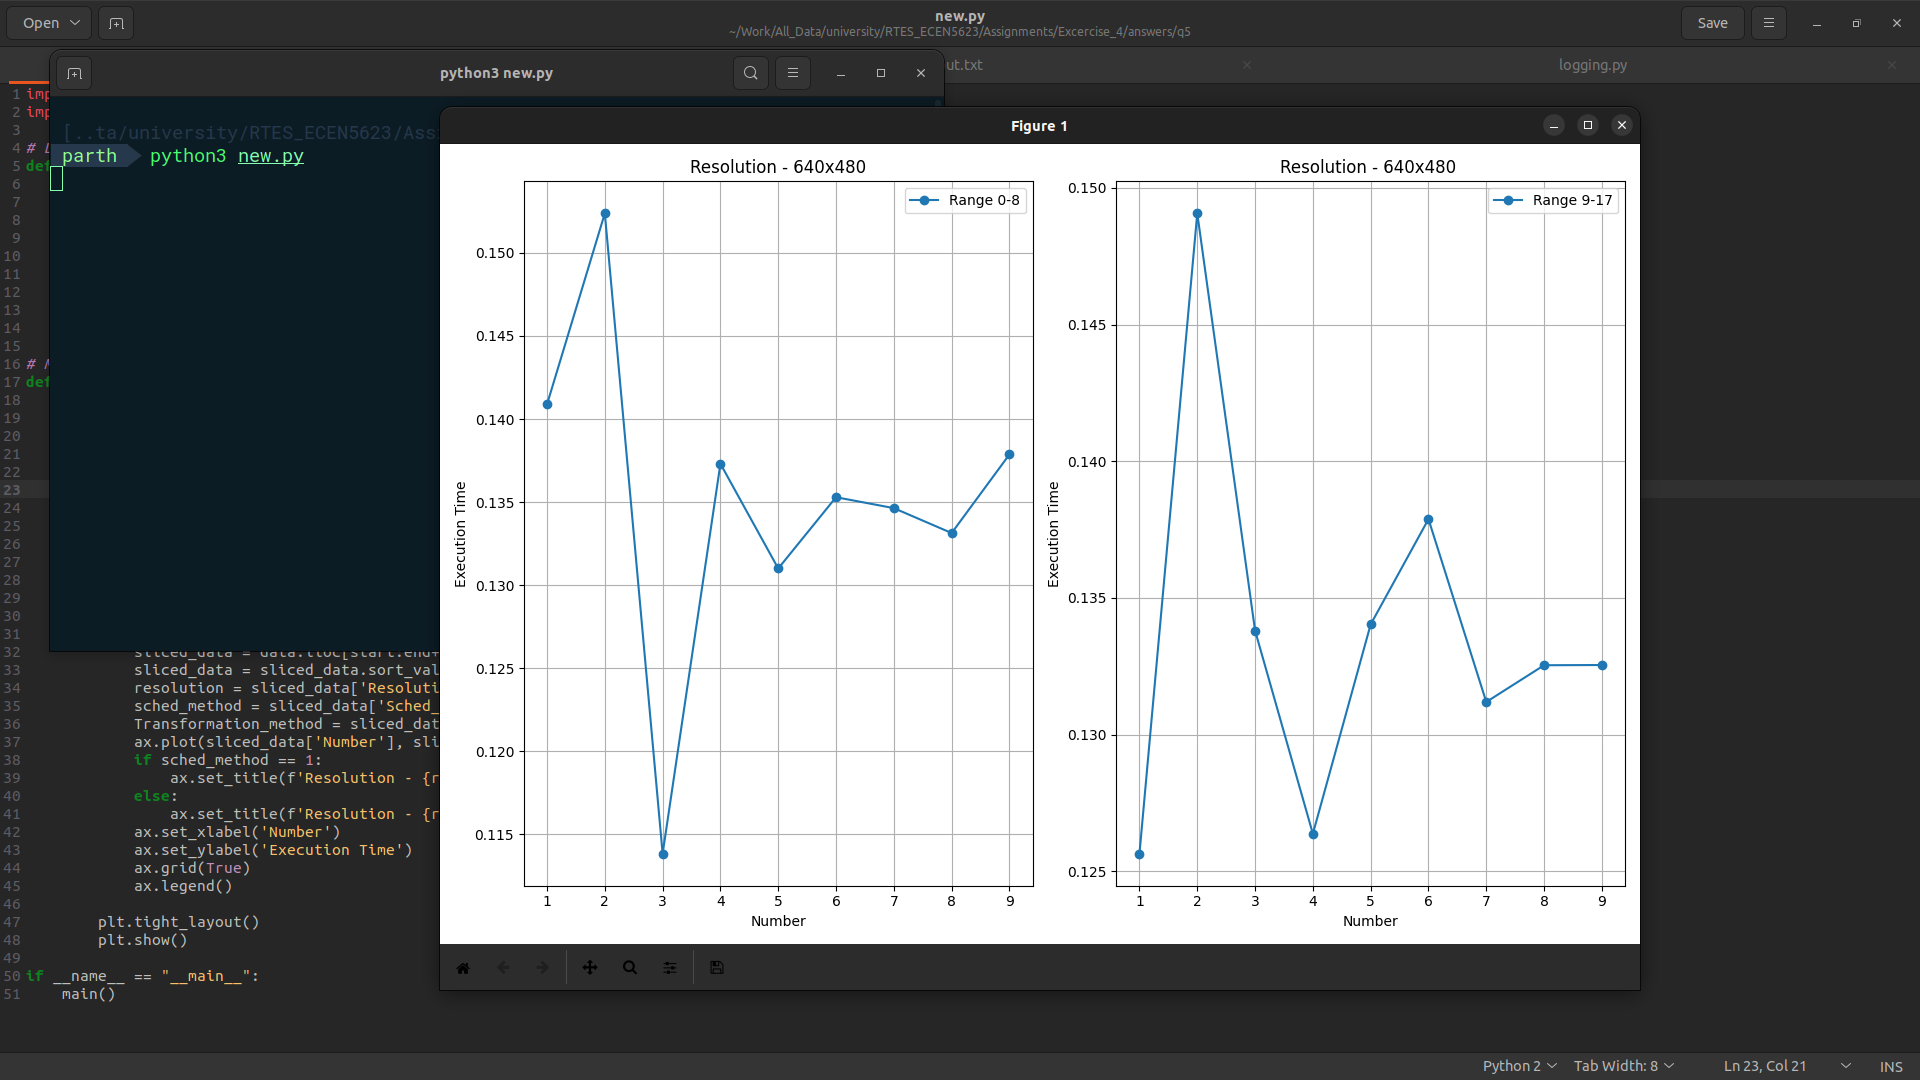
\includegraphics[scale=0.25]{figures/fig1.png}
										\caption{Graph 1}
									\end{figure}
						            \item Graph 2 (Number of Frames \& Execution Time): \begin{figure}[H]
										\centering
										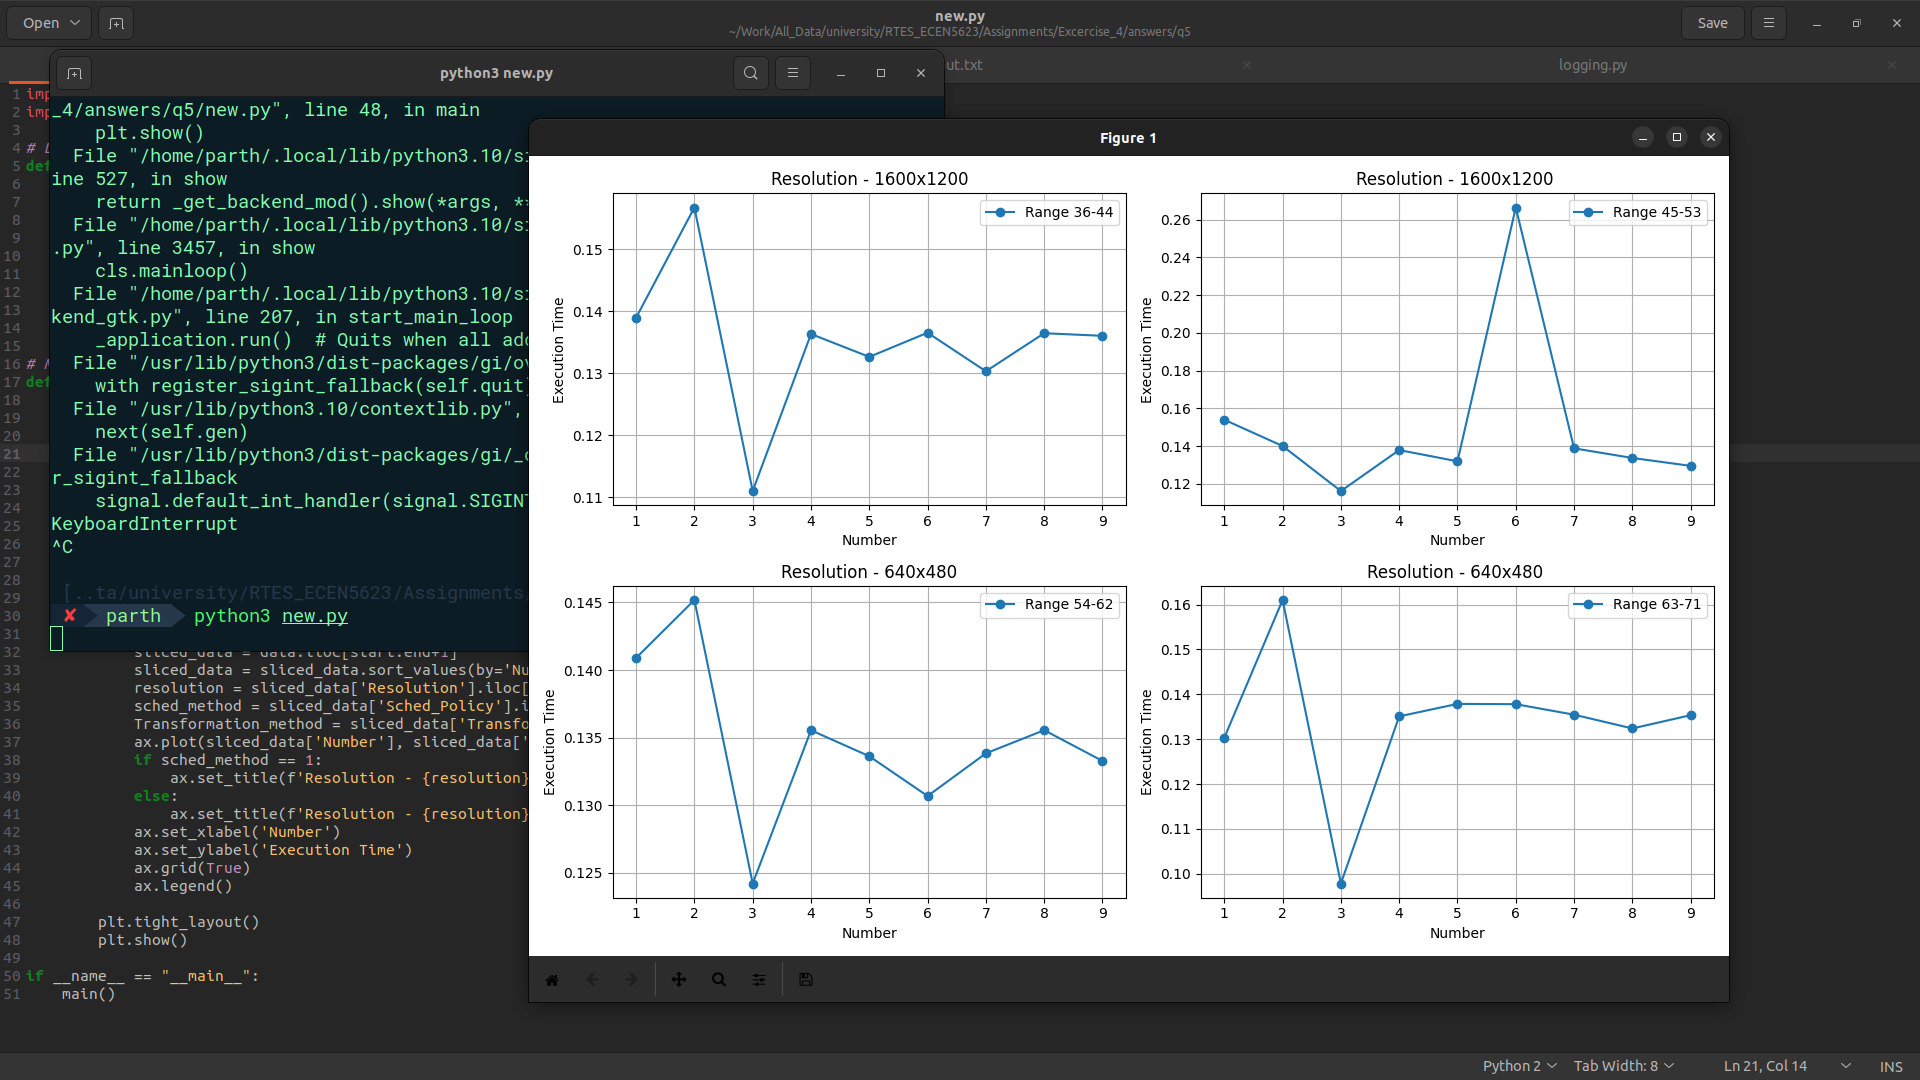
\includegraphics[scale=0.25]{figures/fig2.png}
										\caption{Graph 2}
									\end{figure}
						            \item Graph 2 (Number of Frames \& Execution Time): \begin{figure}[H]
										\centering
										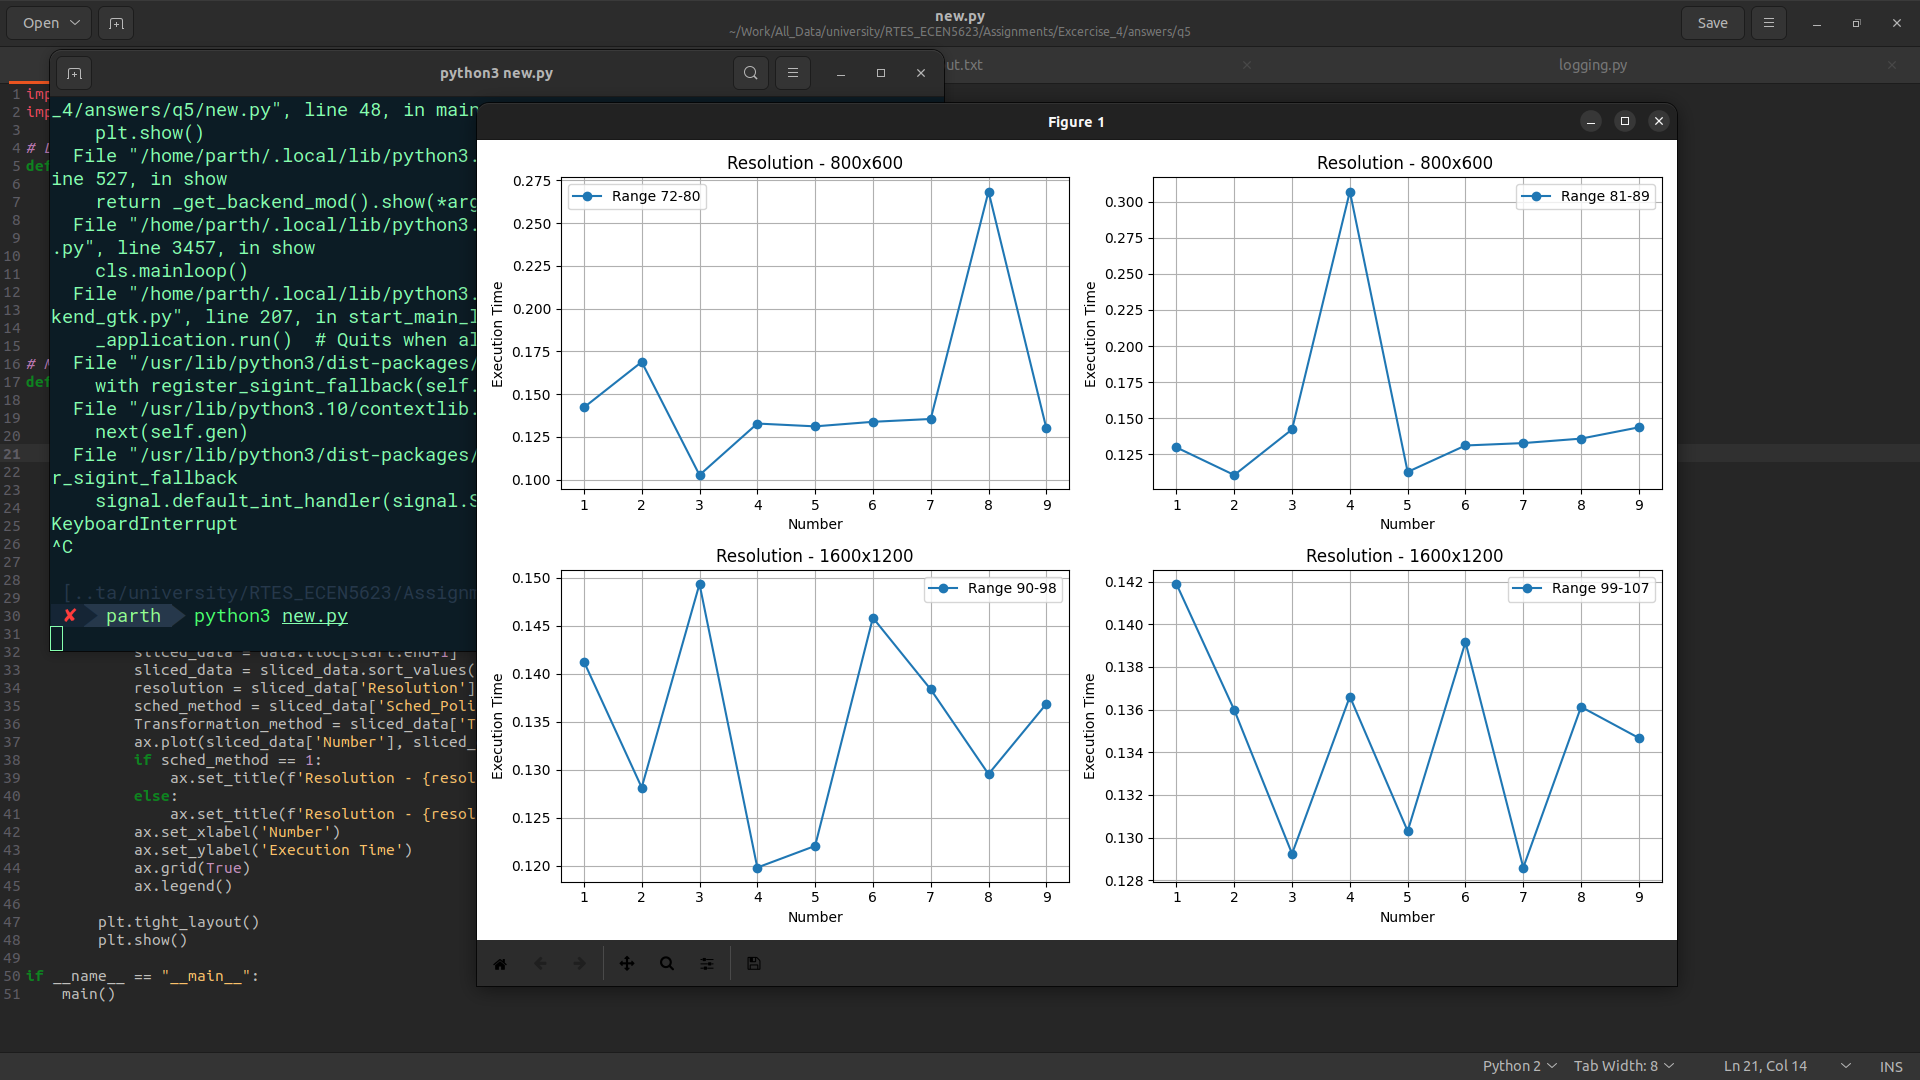
\includegraphics[scale=0.25]{figures/fig3.png}
										\caption{Graph 3}
									\end{figure}
						            \item Graph 2 (Number of Frames \& Execution Time): \begin{figure}[H]
										\centering
										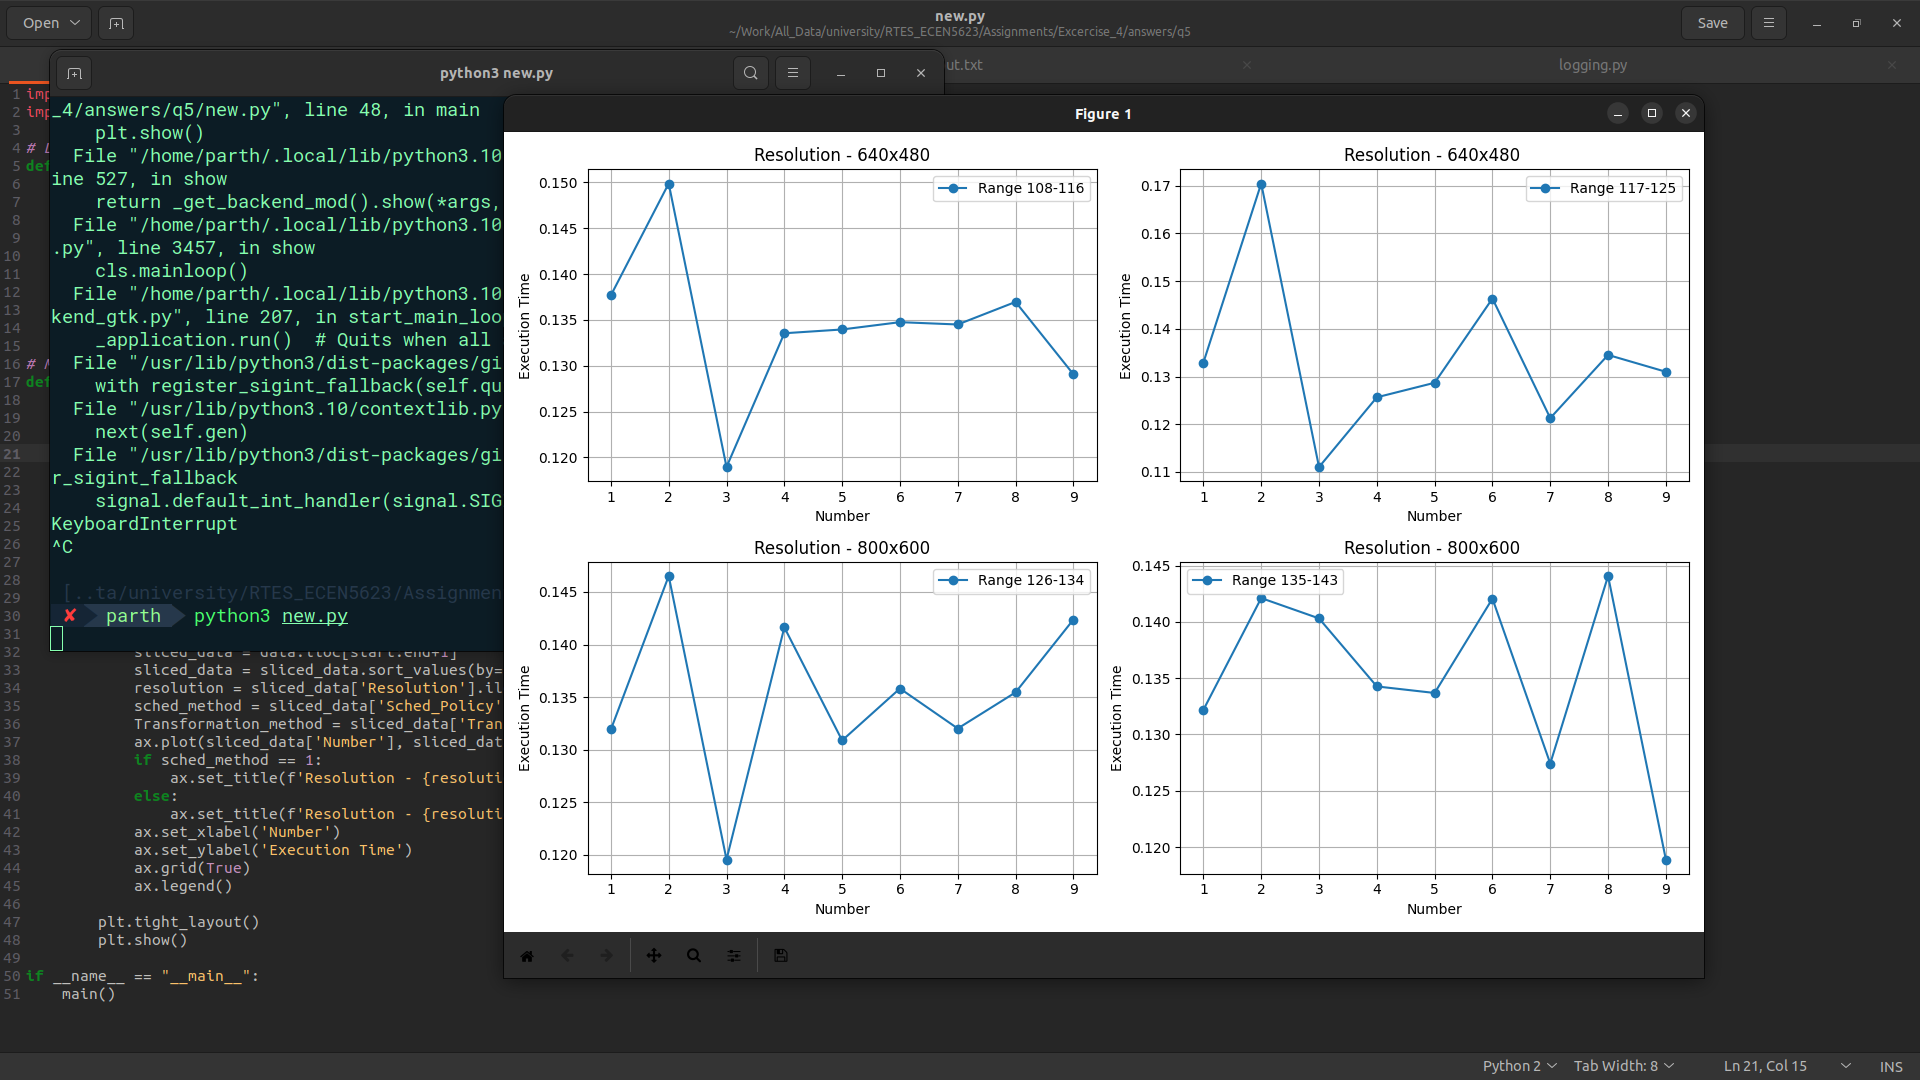
\includegraphics[scale=0.25]{figures/fig4.png}
										\caption{Graph 4}
									\end{figure}
					            \end{itemize}

				      \end{itemize}


			\end{enumerate}


			





	\end{enumerate}

	\begin{enumerate}
		\section{Question 6}
		\item[] \Q [10 points] Demonstrate the results and answer questions from the TA regarding the code
			you developed in \#2, \#3, \#4, and \#5.
	\end{enumerate}



	\section{References}
	\begin{enumerate}
		\item ECEN 5623 Lecture slides material and example codes.
		\item REAL-TIME EMBEDDED COMPONENTS AND SYSTEMS with LINUX and RTOS, Sam Siewert John
		      Pratt (Chapter 6, 7 \& 8).
		\item Exercise 4 requirements included links and documentation.
	\end{enumerate}


\end{qanda}




\vfill
\hrule
\vspace{0.5cm}
\pagebreak
\begin{appendices}
	\section{C/Cpp/Python Code for the Implementation}

	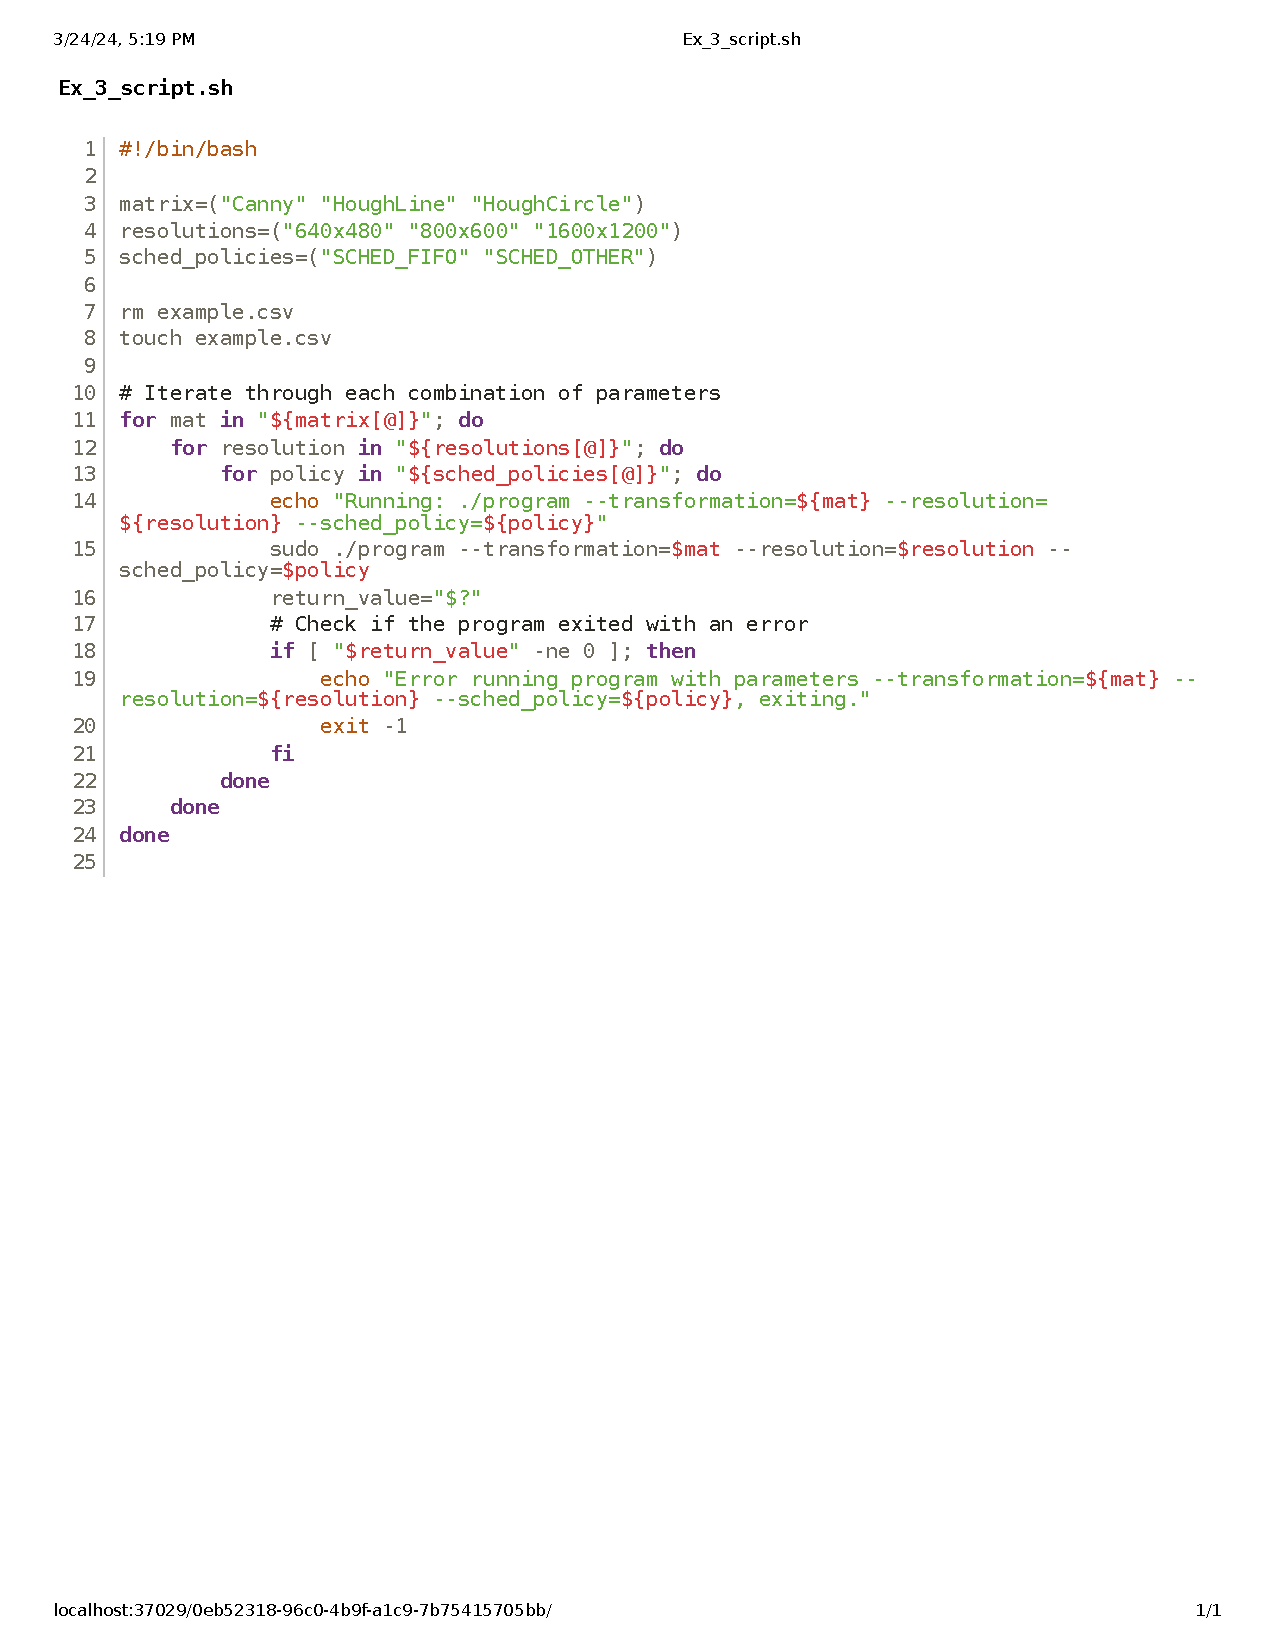
\includepdf[pages=-]{code/Ex_3_script.sh.pdf}
	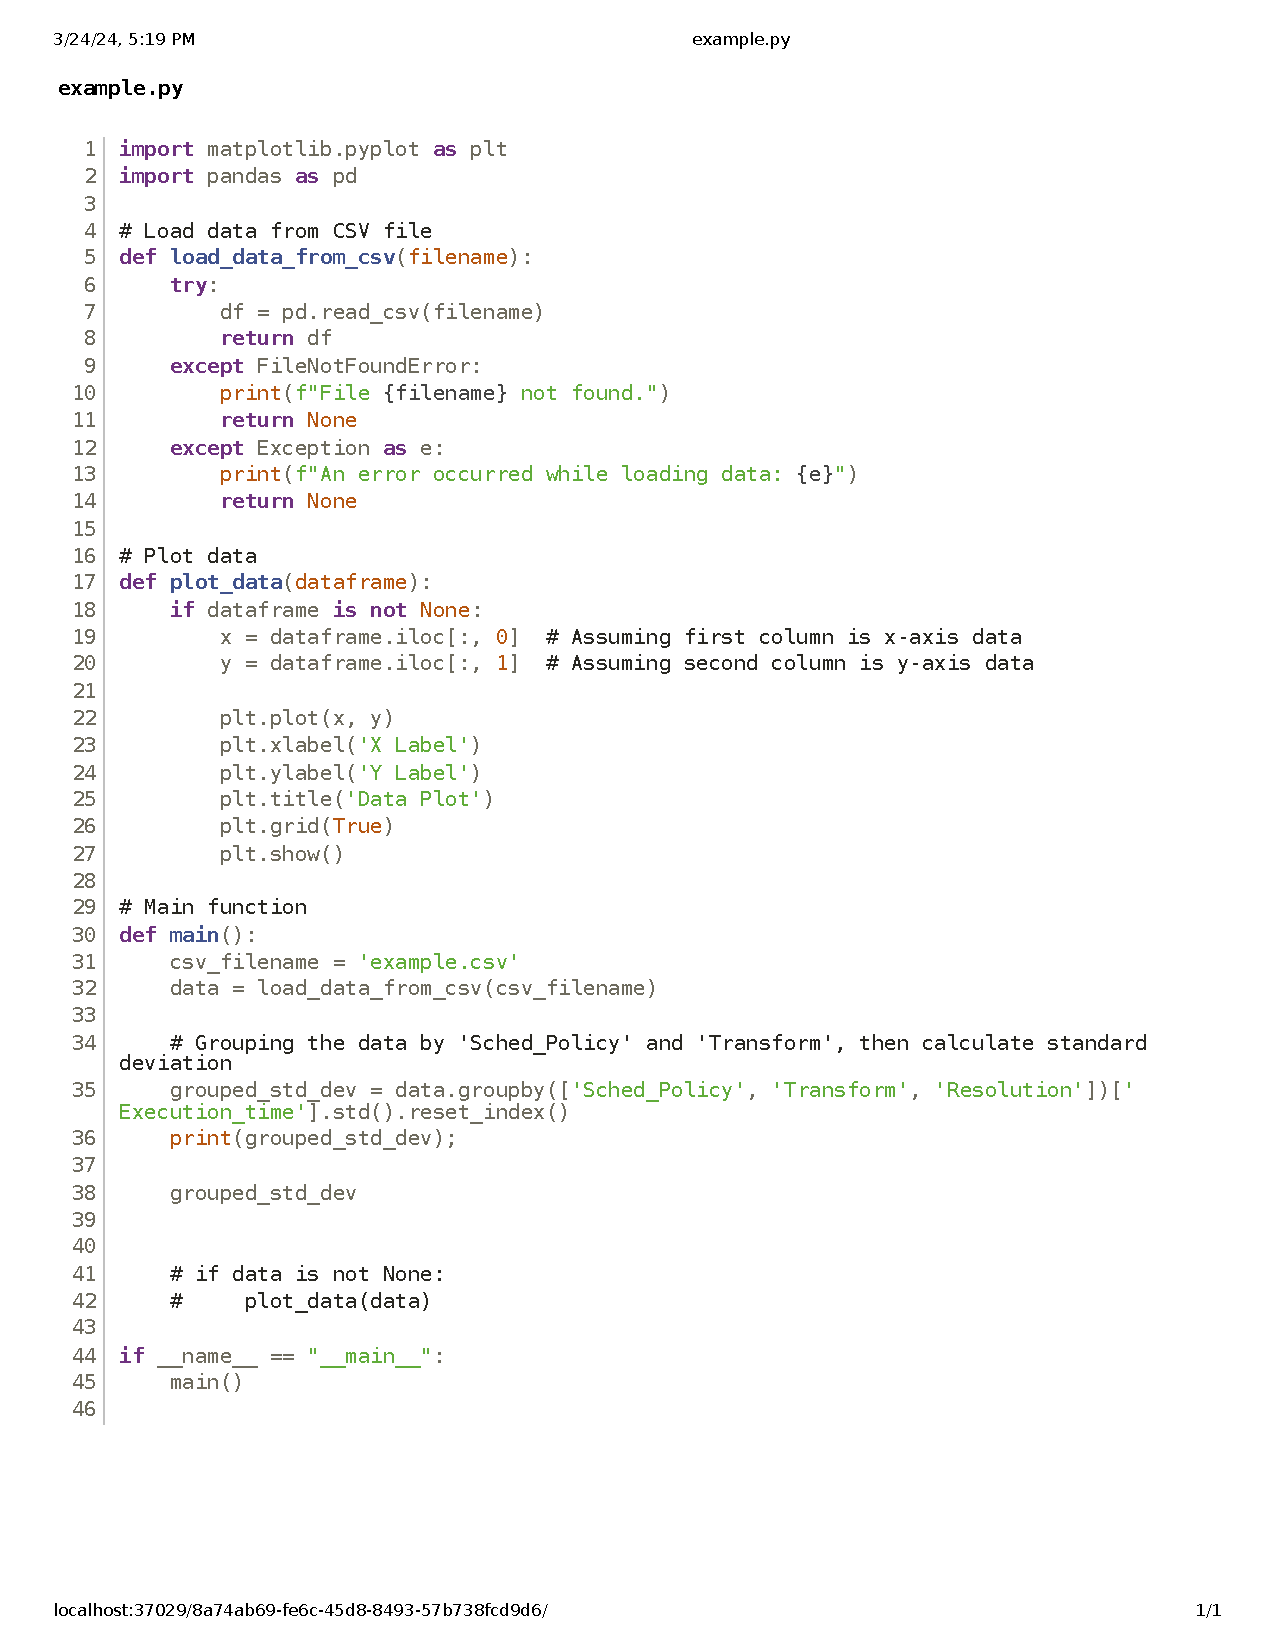
\includepdf[pages=-]{code/example.py.pdf}
	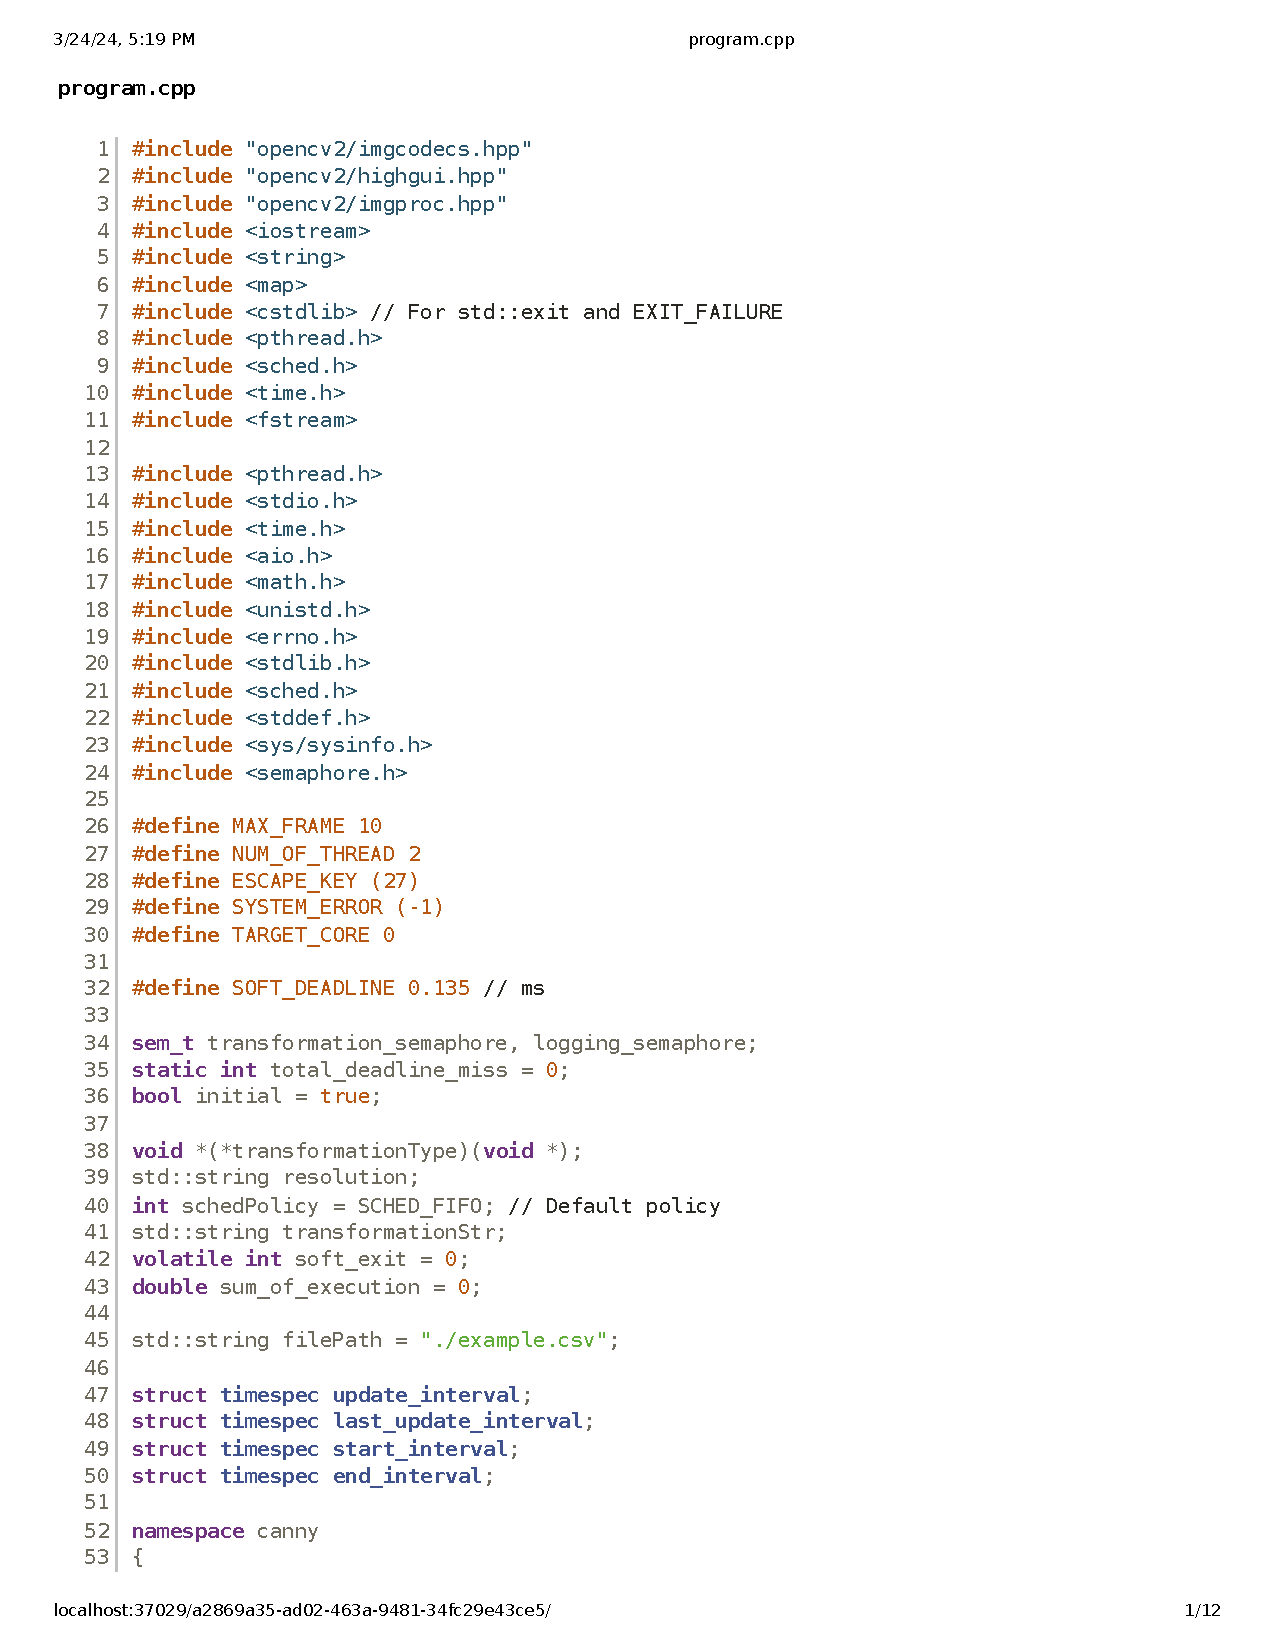
\includepdf[pages=-]{code/program.cpp.pdf}
\end{appendices}


\vspace{1cm}
\hrule
\vspace{0.5cm}


%---------------------------------------------------------------------------
\end{document}
-
